% EDA / CAD technical interview | technology mapping and ECO
% English Beamer interview deck, expanded from user-authored ABC Mapper slides.
% pdfLaTeX; project illustrations are stored in figures/.
% Mapping content preserved; ECO pages are clearly marked as proposed.
% NeoPower is a company project: keep discussion high-level and do not imply that
% every current repository module was personally authored during employment.
%
% Original mapping sequence:
%  1 Cover                 2 Education & Experience   3 Outline
%  4 ABC: Extension       5 ABC: Testing
%  6 NeoPower: Systems    7 NeoPower: Reliability
%  8 Thank You

\documentclass[aspectratio=169,10pt]{beamer}
\usepackage[english]{babel}
\usepackage[utf8]{inputenc}
\usepackage[T1]{fontenc}
\usepackage{lmodern}
\usepackage{amsmath,amssymb}
\usepackage{booktabs}
\usepackage{graphicx}
\usepackage{xcolor}
\usepackage{tikz}
\usetikzlibrary{arrows.meta,positioning,calc,shapes.geometric}
\usepackage{hyperref}
\graphicspath{{./}{figures/}}

% --------- Same Madrid-inspired visual identity as the ABC Mapper deck ---------
\usetheme{Madrid}
\usecolortheme{default}
\definecolor{Ink}{HTML}{243748}
\definecolor{Muted}{HTML}{667B8B}
\definecolor{Accent}{HTML}{347E74}
\definecolor{AccentBlue}{HTML}{507DAD}
\definecolor{SoftMint}{HTML}{E6F4EE}
\definecolor{SoftBlue}{HTML}{E9F2F9}
\definecolor{SoftLilac}{HTML}{F1EEF8}
\definecolor{Paper}{HTML}{FBFCFE}
\definecolor{Divider}{HTML}{D8E4EB}
\setbeamercolor{background canvas}{bg=Paper}
\setbeamercolor{normal text}{fg=Ink}
\setbeamercolor{structure}{fg=Accent}
\setbeamercolor{frametitle}{fg=Ink,bg=SoftBlue}
\setbeamercolor{title}{fg=Ink}
\setbeamercolor{subtitle}{fg=Muted}
\setbeamercolor{block title}{fg=Ink,bg=SoftBlue}
\setbeamercolor{block body}{fg=Ink,bg=white}
\setbeamercolor{item}{fg=Accent}
\setbeamercolor{footline}{fg=Muted,bg=Paper}
\setbeamercolor{panelblue}{fg=Ink,bg=SoftBlue!60}
\setbeamercolor{panelmint}{fg=Ink,bg=SoftMint!72}
\setbeamercolor{panellilac}{fg=Ink,bg=SoftLilac!76}
\setbeamercolor{panelwhite}{fg=Ink,bg=white}
\setbeamerfont{frametitle}{size=\Large,series=\bfseries}
\setbeamerfont{footline}{size=\tiny}
\setbeamertemplate{headline}{}
\setbeamertemplate{navigation symbols}{}
\setbeamertemplate{blocks}[rounded][shadow=false]
\setbeamertemplate{itemize items}[circle]
\setbeamertemplate{footline}{%
  \leavevmode\hbox{%
    \begin{beamercolorbox}[wd=\paperwidth,ht=.30cm,dp=.16cm]{footline}%
      \raggedright\noindent\makebox[\paperwidth][r]{\slideposition\hspace*{.65cm}}
    \end{beamercolorbox}}%
}
\setbeamertemplate{frametitle}{%
  \nointerlineskip
  \begin{beamercolorbox}[wd=\paperwidth,ht=.77cm,dp=.18cm,leftskip=.64cm]{frametitle}%
    \usebeamerfont{frametitle}\insertframetitle%
  % Place links outside the shrinkable frame body to preserve PDF hit areas.
  \begin{tikzpicture}[remember picture,overlay]
    \node[anchor=base east,inner sep=0pt] at
      ([xshift=-.65cm,yshift=-1.50cm]current page.north east)
      {\normalfont\slidenavigation};
  \end{tikzpicture}%
  \end{beamercolorbox}%

}

% --------- Same basic components, plus lightweight reusable panels ---------
\newcommand{\smalllabel}[1]{{\scriptsize\bfseries\color{Accent}\MakeUppercase{#1}}}
\newcommand{\takeaway}[1]{%
  \begin{beamercolorbox}[rounded=true,sep=0.15cm,wd=\linewidth]{block title}%
    \strut\textbf{#1}\strut
  \end{beamercolorbox}%
}
\newcommand{\minibadge}[2]{%
  \tikz[baseline=(badge.base)]\node[fill=#1,rounded corners=3pt,
    inner xsep=6pt,inner ysep=3pt] (badge) {\scriptsize\bfseries #2};%
}
\newcommand{\softpanel}[3]{%
  \begin{beamercolorbox}[rounded=true,sep=0.16cm,wd=\linewidth]{#1}%
    {\small\bfseries\color{Accent}#2}\par\vspace{0.08cm}
    {\small\color{Ink}#3}%
  \end{beamercolorbox}%
}
\newcommand{\smallpanel}[3]{%
  \begin{beamercolorbox}[rounded=true,sep=0.13cm,wd=\linewidth]{#1}%
    {\small\bfseries\color{Accent}#2}\par\vspace{0.06cm}
    {\scriptsize\color{Ink}#3}%
  \end{beamercolorbox}%
}
\newcommand{\outlinecard}[4]{%
  \begin{beamercolorbox}[rounded=true,sep=0.17cm,wd=\linewidth]{#1}%
    \begin{minipage}[c]{0.34\linewidth}
      {\normalsize\bfseries #2}\par\vspace{0.03cm}
      {\scriptsize\color{Accent}#3}
    \end{minipage}\hfill%
    \begin{minipage}[c]{0.63\linewidth}
      {\small #4}
    \end{minipage}%
  \end{beamercolorbox}%
}
\newcommand{\gate}[3]{%
  \begin{beamercolorbox}[rounded=true,sep=0.15cm,wd=\linewidth]{panelwhite}%
    {\small\bfseries\color{Accent}#1\quad #2}\par\vspace{0.07cm}
    {\scriptsize\color{Muted}#3}%
  \end{beamercolorbox}%
}


% --- Custom slide components: same color palette and structure as the template ---
% Reserved image areas can be replaced by \\includegraphics[width=...]{your_image}.
\newcommand{\figurespace}[3]{%
  \begin{tikzpicture}
    \node[draw=AccentBlue!50,dashed,rounded corners=3pt,fill=white,
      text width=.90\linewidth,minimum height=#1,align=center,inner sep=5pt] {%
      {\scriptsize\bfseries\color{AccentBlue}FIGURE SPACE}\\[3mm]
      {\normalsize\bfseries\color{Muted}#2}\\[2mm]
      {\scriptsize\color{Muted}#3}%
    };
  \end{tikzpicture}%
}
\newcommand{\statcard}[2]{%
  \begin{beamercolorbox}[rounded=true,sep=.13cm,wd=\linewidth]{panelwhite}
    {\Large\bfseries\color{Ink}#1}\par
    {\scriptsize\color{Muted}#2}
  \end{beamercolorbox}%
}
\newcommand{\scitem}[2]{%
  \begin{beamercolorbox}[rounded=true,sep=.14cm,wd=\linewidth]{panelblue}
    {\small\bfseries\color{Accent}#1}\par\vspace{.06cm}
    {\scriptsize #2}
  \end{beamercolorbox}%
}

% Reusable visual placeholder from the original portfolio template.
% Mapping / ECO research figures elsewhere in this deck continue to use \figurespace.
\providecommand{\aiplaceholder}[3]{}
\renewcommand{\aiplaceholder}[3]{%
  \par\noindent
  \begin{tikzpicture}
    \node[draw=AccentBlue!55,dashed,line width=0.6pt,
      rounded corners=4pt,fill=SoftBlue!35,
      text width=\dimexpr\linewidth-0.82cm\relax,
      minimum height=#1,inner xsep=0.40cm,inner ysep=0.12cm,
      outer sep=0pt,align=center] {%
      {\small\bfseries\color{AccentBlue}IMAGE PLACEHOLDER}\par
      \vspace{0.12cm}
      {\small\color{Ink}#2\par}
      \vspace{0.10cm}
      {\scriptsize\ttfamily\color{Muted}\detokenize{#3}\par}%
    };
  \end{tikzpicture}\par
}


\title[CAD Technical Interview]{EDA / CAD Engineering Projects}
\subtitle{Selected Research and Engineering Projects}
\author{Yu-Jui (Stanley) Liang}
\institute{National Taiwan University}
\date{}

% Unified S1-S5 card height; keeps five candidates easy to compare.
\newcommand{\ecostrategycard}[3]{%
  \begin{beamercolorbox}[rounded=true,sep=.20cm,wd=\linewidth]{#1}%
    \begin{minipage}[c][1.43cm][c]{\dimexpr\linewidth-.40cm\relax}
      {\normalsize\bfseries\color{Accent}#2}\par\vspace{.11cm}
      {\small\raggedright\hyphenpenalty=10000\exhyphenpenalty=10000 #3\par}
    \end{minipage}%
  \end{beamercolorbox}%
}


% Navigation shares the subtitle row; the footer reserves a fixed right margin.
% Stable summary-N and detail-topic labels support links in both directions.
\newcommand{\slidenavigation}{}
\newcommand{\slideposition}{}
\newcommand{\slidesubtitle}[1]{%
  \smalllabel{#1}%
}
\setbeamercolor{button}{fg=Accent,bg=SoftMint}
\setbeamercolor{button border}{fg=Accent!50}
\setbeamerfont{button}{size=\scriptsize}

\begin{document}
% 18 summary pages: portfolio, mapping cover + content, ECO cover + content.


% ============================================================
% No duplicate project listing on this cover; see slide 4.
% ============================================================
% ------------------------------------------------------------------------
% SLIDE 1 / 18 | Portfolio Cover
% ------------------------------------------------------------------------
{\setbeamertemplate{footline}{}
\renewcommand{\slidenavigation}{\hyperlink{details-index}{\beamerbutton{Details index}}}
\renewcommand{\slideposition}{Summary 1 / 18}
\begin{frame}[plain,label=summary-1]
  \vspace*{1.65cm}
  \smalllabel{CAD Engineering Technical Interview}\par
  \vspace{0.51cm}
  {\raggedright\fontsize{21}{27}\selectfont\bfseries\color{Ink}
    EDA / CAD Engineering Projects\par}
  \vspace{0.29cm}
  {\normalsize\color{Muted}Logic Synthesis \enspace / \enspace Physical Design \enspace / \enspace Timing ECO \enspace / \enspace CAD Flow Automation\par}
  \vspace{0.70cm}
  {\Large\bfseries\color{Ink}Yu-Jui (Stanley) Liang}\par
  \vspace{0.10cm}
  {\normalsize\color{Muted}M.S. Candidate, Data Science Master Degree Program\par}
  {\normalsize\color{Muted}National Taiwan University\par}
  \vskip0pt plus 1filll
  {\color{Accent}\rule{\textwidth}{0.7pt}}\par
  \vspace{0.16cm}
  {\small\href{mailto:liangyujui@gmail.com}{liangyujui@gmail.com}
     \quad | \quad
     \href{https://www.linkedin.com/in/yu-jui-liang-735a57316}{linkedin.com/in/yu-jui-liang-735a57316}\par}
  \vspace*{0.55cm}
\end{frame}}

% ============================================================
% ============================================================
% ------------------------------------------------------------------------
% SLIDE 2 / 18 | Education & Research Interests
% ------------------------------------------------------------------------
\renewcommand{\slidenavigation}{\hyperlink{details-index}{\beamerbutton{Details index}}}
\renewcommand{\slideposition}{Summary 2 / 18}
\begin{frame}[label=summary-2]{Education \& Research Interests}
  \vspace{0.05cm}
  \slidesubtitle{01 / Profile}\par\vspace{0.10cm}
  \vfill
  \begin{columns}[T,onlytextwidth]
    \begin{column}{0.49\textwidth}
      \begin{beamercolorbox}[rounded=true,sep=0.20cm,wd=\linewidth]{panelblue}
        {\large\bfseries\color{AccentBlue}Education}\par
        \vspace{0.14cm}
        {\normalsize\bfseries National Taiwan University}\par
        {\normalsize M.S. Candidate, Data Science Master Degree Program}\par
        {\small\color{Muted}Sep. 2025 -- Expected Jun. 2027}\par
        \vspace{0.23cm}
        {\normalsize\bfseries National Chengchi University}\par
        {\normalsize B.S. in Computer Science}\par
        {\normalsize Double Major in Electronic Physics}\par
        {\small\color{Muted}Sep. 2021 -- Jun. 2025}
      \end{beamercolorbox}
    \end{column}
    \begin{column}{0.49\textwidth}
      \begin{beamercolorbox}[rounded=true,sep=0.20cm,wd=\linewidth]{panelmint}
        {\large\bfseries\color{Accent}Research Interests}\par
        \vspace{0.15cm}
        {\normalsize\bfseries EDA / CAD \& VLSI Design Automation}\par
        \vspace{0.09cm}
        {\normalsize Logic Synthesis}\par
        {\normalsize Technology Mapping}\par
        {\normalsize Static Timing Analysis}\par
        {\normalsize Timing Closure}\par
        {\normalsize Physical Design}\par
        {\normalsize Incremental ECO}\par
        {\normalsize PPA}\par
        \vspace{0.15cm}
        {\normalsize\bfseries Algorithm \& Software Development}\par
        \vspace{0.09cm}
        {\normalsize C++ / Python / Tcl Flow Automation}\par
      \end{beamercolorbox}
    \end{column}
  \end{columns}
  \vfill
\end{frame}

% ============================================================
% ============================================================
% ------------------------------------------------------------------------
% SLIDE 3 / 18 | Professional Software Engineering Experience
% ------------------------------------------------------------------------
\renewcommand{\slidenavigation}{\hyperlink{details-index}{\beamerbutton{Details index}}}
\renewcommand{\slideposition}{Summary 3 / 18}
\begin{frame}[label=summary-3]{Professional Software Engineering Experience}
  \vspace{0.04cm}
  \slidesubtitle{02 / Work Experience}\par\vspace{0.10cm}
  \takeaway{Software development, simulation, and validation experience in R\&D environments.}
  \vfill

  \begin{beamercolorbox}[rounded=true,sep=0.19cm,wd=\linewidth]{panelblue}
    {\normalsize\bfseries\color{Ink}AIMobile Co., Ltd. (Inventec Group)}\hfill
    {\scriptsize\color{Muted}Apr. 2025 -- Jul. 2025}\par
    \vspace{0.07cm}
    {\small\bfseries\color{AccentBlue}Contract Software Engineer}\par
    \vspace{0.14cm}
    {\small\color{Ink}Contributed to software development and system integration in an R\&D environment.}\par
    \vspace{0.08cm}
    {\small\color{Ink}Supported debugging and functional validation across software modules.}\par
  \end{beamercolorbox}

  \vfill
  \begin{beamercolorbox}[rounded=true,sep=0.19cm,wd=\linewidth]{panelmint}
    {\normalsize\bfseries\color{Ink}Neopower Technologies Co., Ltd.}\hfill
    {\scriptsize\color{Muted}Jun. 2023 -- Mar. 2025}\par
    \vspace{0.07cm}
    {\small\bfseries\color{Accent}Contract Software Engineer}\par
    \vspace{0.14cm}
    {\small\color{Ink}Developed a custom system simulator to reproduce operational and error scenarios.}\par
    \vspace{0.08cm}
    {\small\color{Ink}Performed regression checks, log analysis, and customer-side A/B validation.}\par
  \end{beamercolorbox}
  \vfill
\end{frame}

% ============================================================
% ============================================================
% ------------------------------------------------------------------------
% SLIDE 4 / 18 | Selected Projects & Discussion Topics
% ------------------------------------------------------------------------
\renewcommand{\slidenavigation}{\hyperlink{details-index}{\beamerbutton{Details index}}}
\renewcommand{\slideposition}{Summary 4 / 18}
\begin{frame}[label=summary-4]{Selected Projects \& Discussion Topics}
  \vspace{0.03cm}
  \slidesubtitle{03 / Project Overview}\par\vspace{0.11cm}
  \vfill
  \begin{beamercolorbox}[rounded=true,sep=0.20cm,wd=\linewidth]{panelblue}
    {\small\bfseries\color{AccentBlue}01 \quad Master's Research --- Logic Synthesis (Front End)}\par
    \vspace{0.05cm}
    {\normalsize\bfseries Joint Single- and Multi-Output Cell Mapping via Differentiable Optimization}\par
    \vspace{0.07cm}
    {\small EDA Tool Development \quad / \quad Boolean Matching \quad / \quad Area--Delay Optimization}
  \end{beamercolorbox}
  \vfill
  \begin{beamercolorbox}[rounded=true,sep=0.20cm,wd=\linewidth]{panellilac}
    {\small\bfseries\color{Accent}02 \quad ICCAD 2025 Problem C --- CAD Methodology (Back End)}\par
    \vspace{0.05cm}
    {\normalsize\bfseries STA-Driven Incremental Timing ECO Search}\par
    \vspace{0.07cm}
    {\small OpenROAD / OpenSTA \quad / \quad Python--Tcl Flow Automation \quad / \quad Heuristic PPA Search}
  \end{beamercolorbox}
  \vfill
\end{frame}

% ==============================================================
% Main technical contents retained from the uploaded Beamer source.
% The 15-minute and 30-minute versions allocate equal time to
% Project 01 (Mapping) and Project 02 (STA-Driven ECO Optimization).
% ==============================================================

% ============================================================
% PROJECT 01 SECTION OPENER | same cover pattern as Project 02
% ============================================================
% ------------------------------------------------------------------------
% SLIDE 5 / 18 | Project 01 Opener: Joint SO / MO Cell Mapping
% ------------------------------------------------------------------------
{\setbeamertemplate{footline}{}
\renewcommand{\slidenavigation}{\hyperlink{details-index}{\beamerbutton{Details index}}}
\renewcommand{\slideposition}{Summary 5 / 18}
\begin{frame}[plain,label=summary-5]
  \vfill
  \smalllabel{Project 01 / Master's Research / Logic Synthesis}\par
  \vspace{.40cm}
  \begin{beamercolorbox}[rounded=true,sep=.25cm,wd=\linewidth]{panelblue}
    {\fontsize{13.6}{17}\selectfont\bfseries\color{Ink}
    \mbox{Technology Mapping for Multi-Output Standard Cells}\par}
    \vspace{.14cm}
    {\normalsize\color{Ink}
      FA/HA cells over a shared input boundary\par}
  \end{beamercolorbox}
  \vspace{.80cm}
  \smalllabel{My Proposed Approach}\par
  \vspace{.17cm}
  {\fontsize{18}{23}\selectfont\bfseries\color{Accent}
    Joint Single- and Multi-Output Cell Mapping\\
    via Differentiable Optimization\par}
  \vspace{.18cm}
  {\small\color{Muted}
    MO candidate discovery in ABC, area-aware MILP pre-selection, and a mapping optimizer adapted from prior work.\par}
  \vfill
\end{frame}}

% ------------------------------------------------------------------------
% SLIDE 6 / 18 | ABC Mapper: SO Technology Mapper Baseline
% ------------------------------------------------------------------------
\renewcommand{\slidenavigation}{\hyperlink{details-index}{\beamerbutton{Details index}}\hspace{.12cm}\hyperlink{detail-dc-abc}{\beamerbutton{DC vs ABC}}}
\renewcommand{\slideposition}{Summary 6 / 18}
\begin{frame}[label=summary-6]{ABC Mapper: SO Technology Mapper Baseline}
  \vspace{.02cm}
  \slidesubtitle{01 / Baseline Mapping}\par\vspace{.08cm}
  \takeaway{The open-source ABC synthesis framework primarily targets single-output cell mapping, leaving joint FA/HA output mapping unsupported in the baseline flow.}
  \vspace{.08cm}
  \begin{center}
    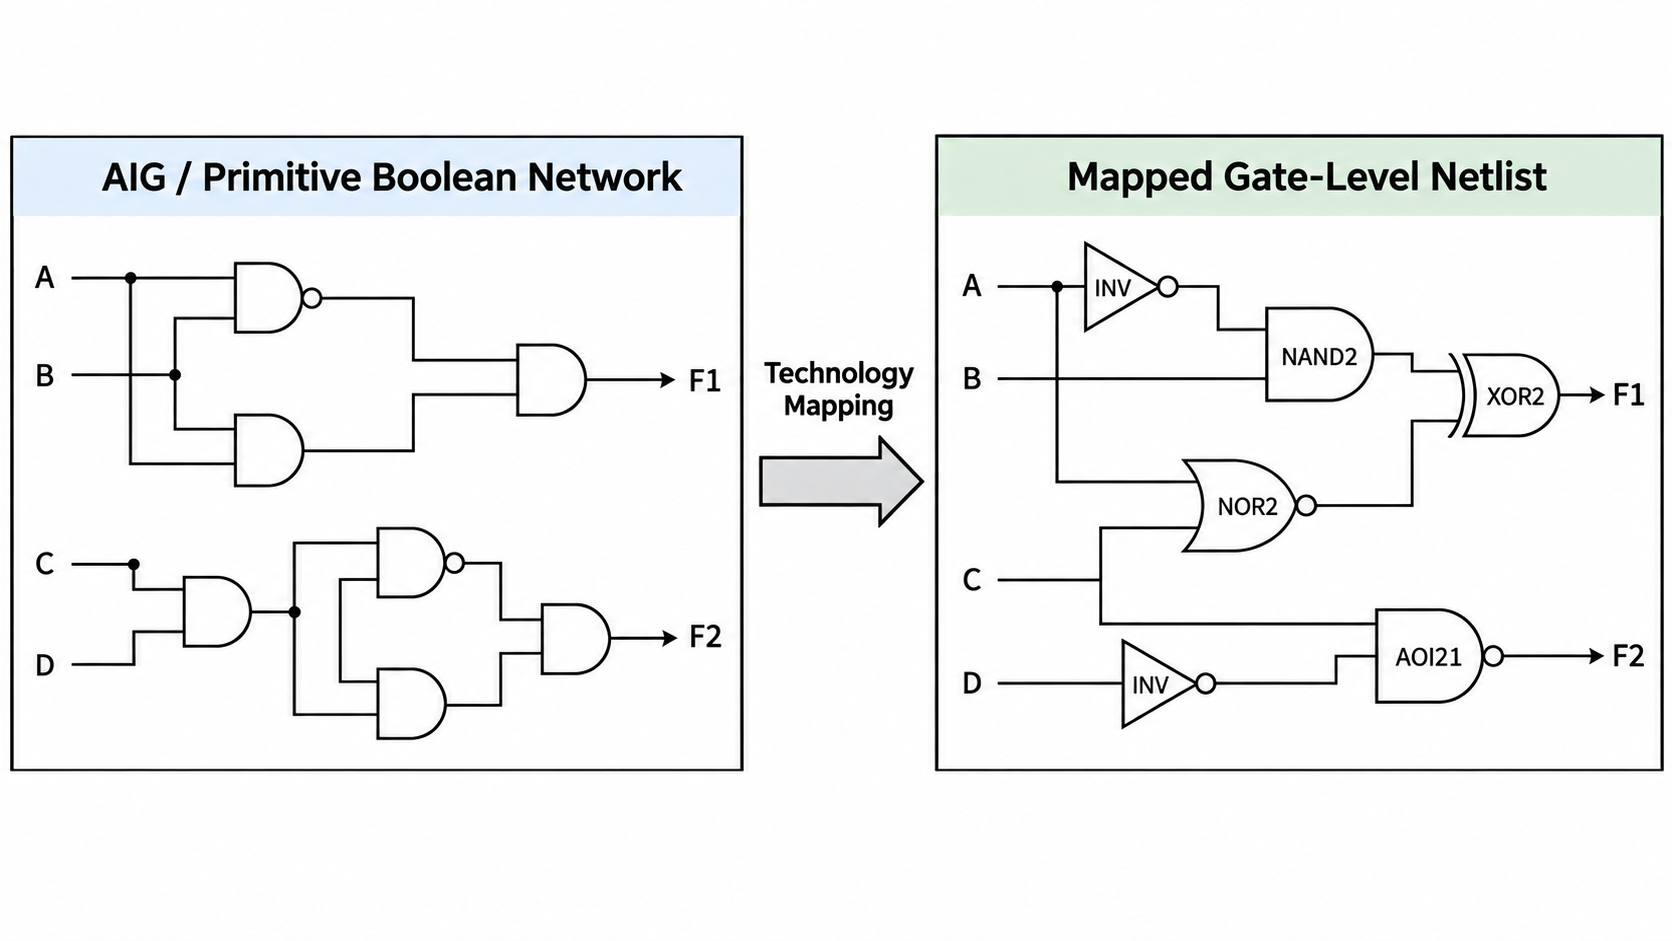
\includegraphics[width=\linewidth,height=4.22cm,keepaspectratio,trim=8bp 158bp 8bp 125bp,clip]{aig-technology-mapping.png}\par
    \vspace{.06cm}
    {\small\color{Muted}Same Boolean behavior, realized with ASAP7 7nm library cells.}
  \end{center}
\end{frame}


% SLIDE 7 / 18 | Single-output vs multi-output motivation
% ------------------------------------------------------------------------
\renewcommand{\slidenavigation}{\hyperlink{details-index}{\beamerbutton{Details index}}\hspace{.12cm}\hyperlink{summary-6}{\beamerbutton{SO baseline}}}
\renewcommand{\slideposition}{Summary 7 / 18}
\begin{frame}[label=summary-7]{Single-Output vs Multi-Output Cell Mapping}
  \slidesubtitle{02 / Motivation}\par\vspace{.10cm}
  \takeaway{A shared FA cell can implement two output functions over the same input boundary.}
  \vfill
  \begin{columns}[T,onlytextwidth]
    \begin{column}{.49\textwidth}
      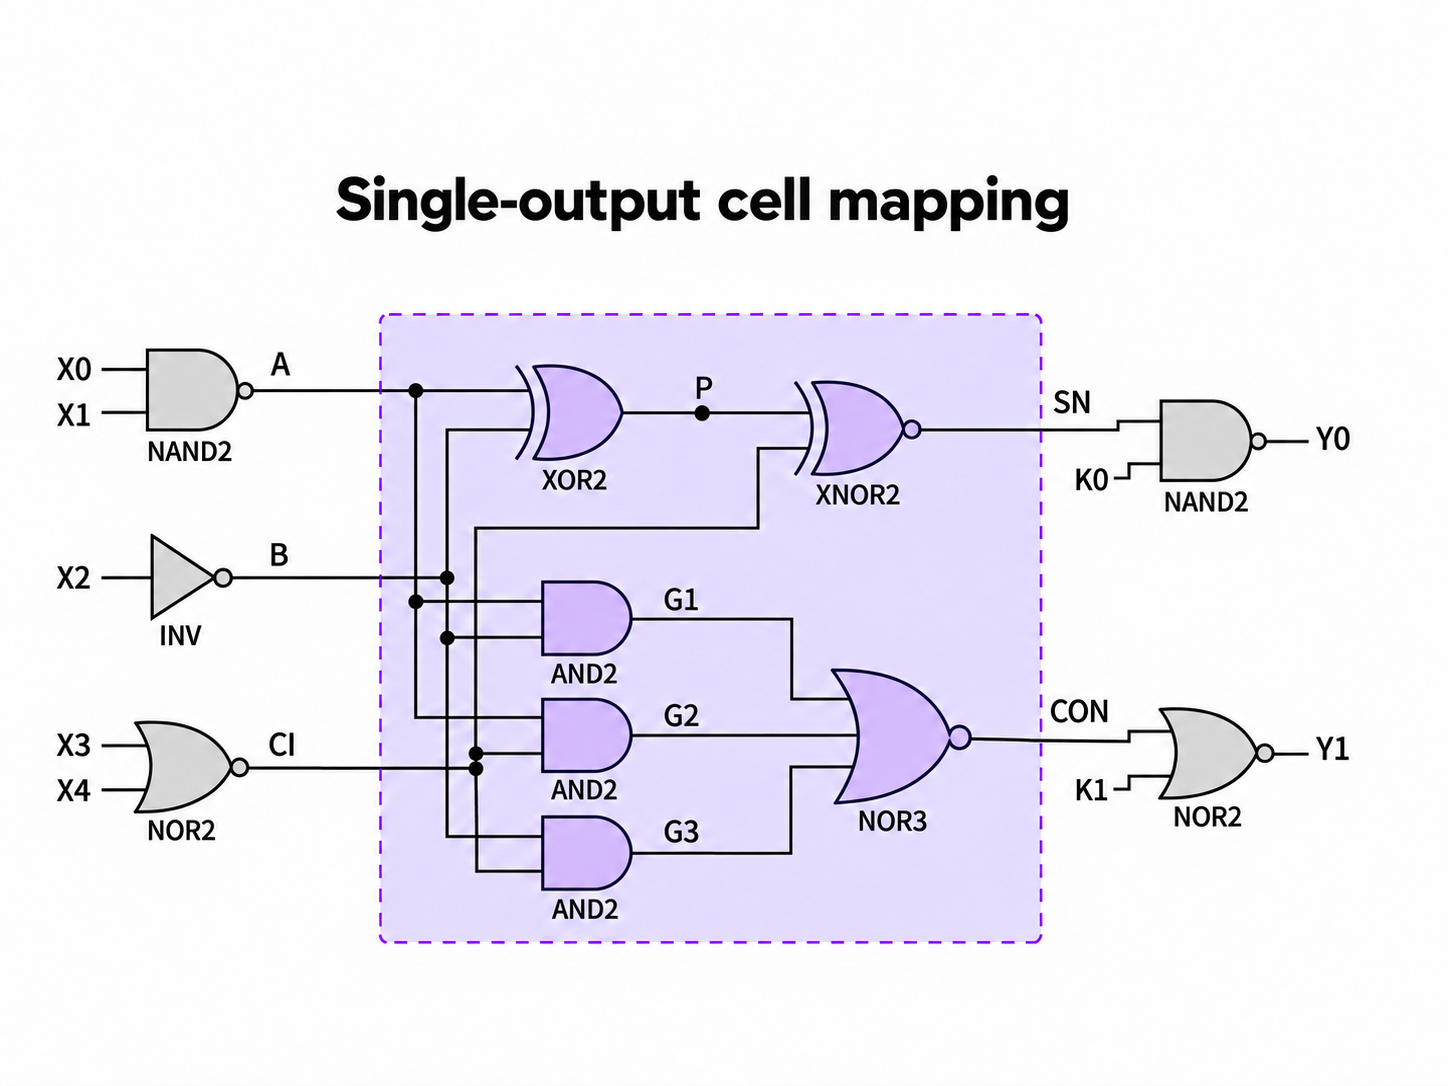
\includegraphics[width=\linewidth,height=3.65cm,keepaspectratio,trim=0 105bp 0 250bp,clip]{single-output-cell-mapping.png}
    \end{column}
    \begin{column}{.49\textwidth}
      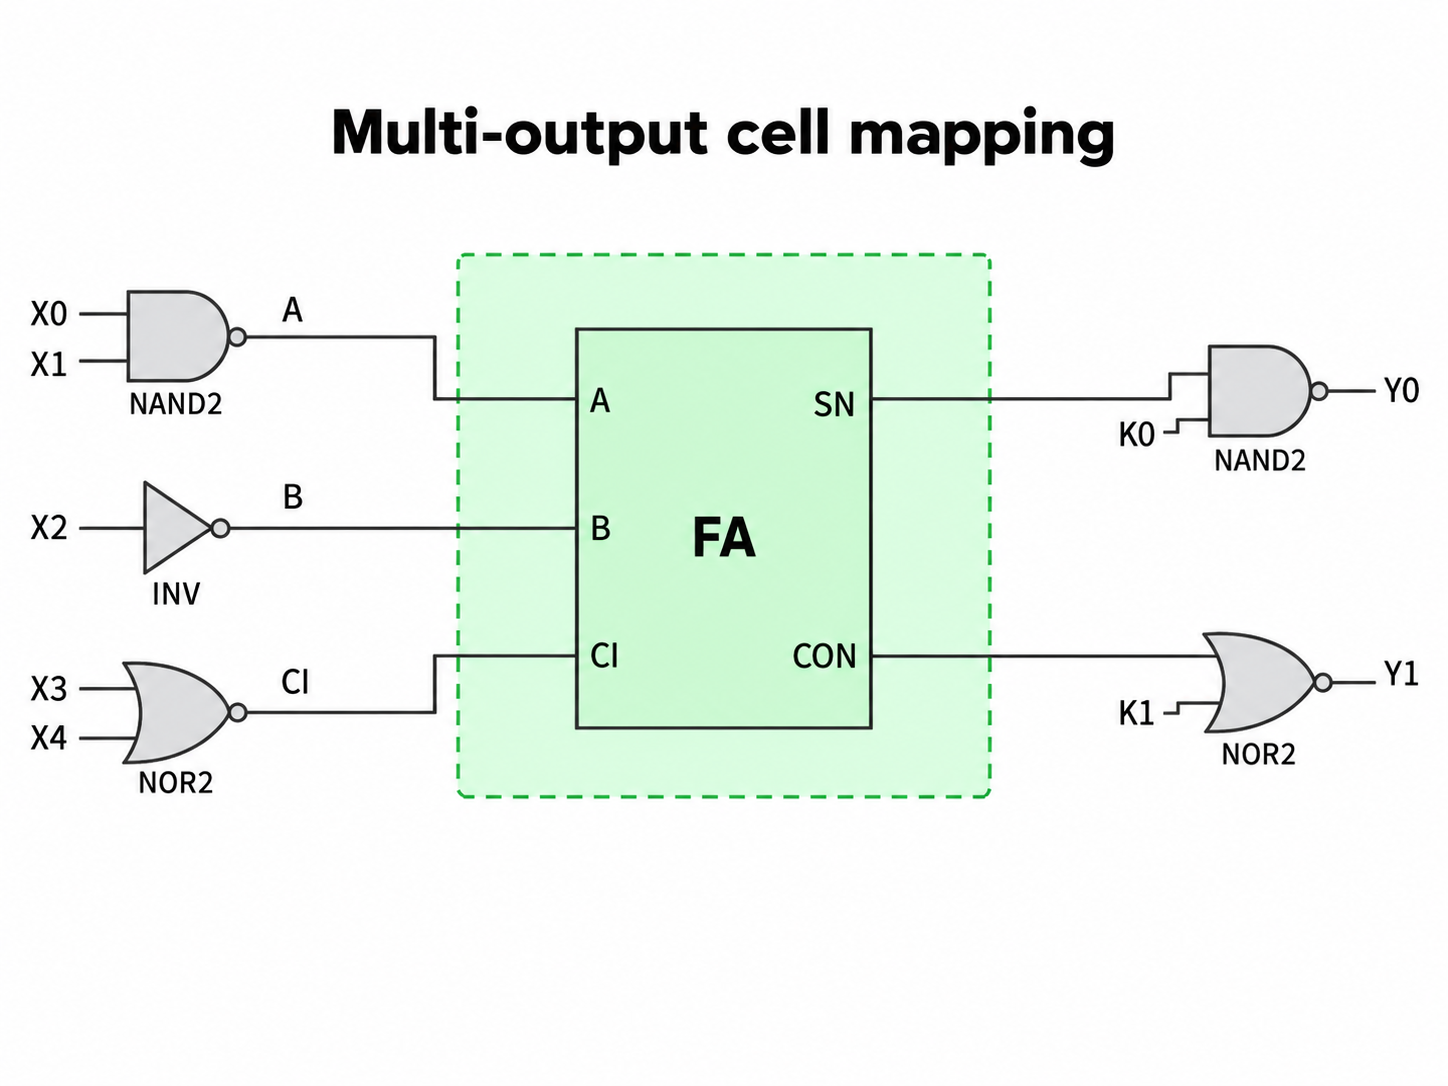
\includegraphics[width=\linewidth,height=3.65cm,keepaspectratio,trim=0 180bp 0 175bp,clip]{multi-output-cell-mapping.png}
    \end{column}
  \end{columns}
  \vspace{.12cm}
  {\small Independent MO discovery exposes joint output matches beyond SO-oriented cut retention.}
  \vfill
\end{frame}


% ------------------------------------------------------------------------
% SLIDE 8 / 18 | Joint SO / MO Mapping: Research Pipeline
% ------------------------------------------------------------------------
\renewcommand{\slidenavigation}{\hyperlink{details-index}{\beamerbutton{Details index}}\hspace{.12cm}\hyperlink{summary-6}{\beamerbutton{SO baseline}}\hspace{.12cm}\hyperlink{summary-11}{\beamerbutton{Optimizer integration}}}
\renewcommand{\slideposition}{Summary 8 / 18}
\begin{frame}[shrink=8,label=summary-8]{Joint SO / MO Mapping: Research Pipeline}
  \vspace{.02cm}
  \slidesubtitle{03 / Research Scope}\par\vspace{.08cm}
  \takeaway{We extend the ABC Mapper with multi-output candidate discovery and area-aware MILP selection, while preserving the original single-output mapping path.}
  \vspace{.16cm}
  \begin{center}
    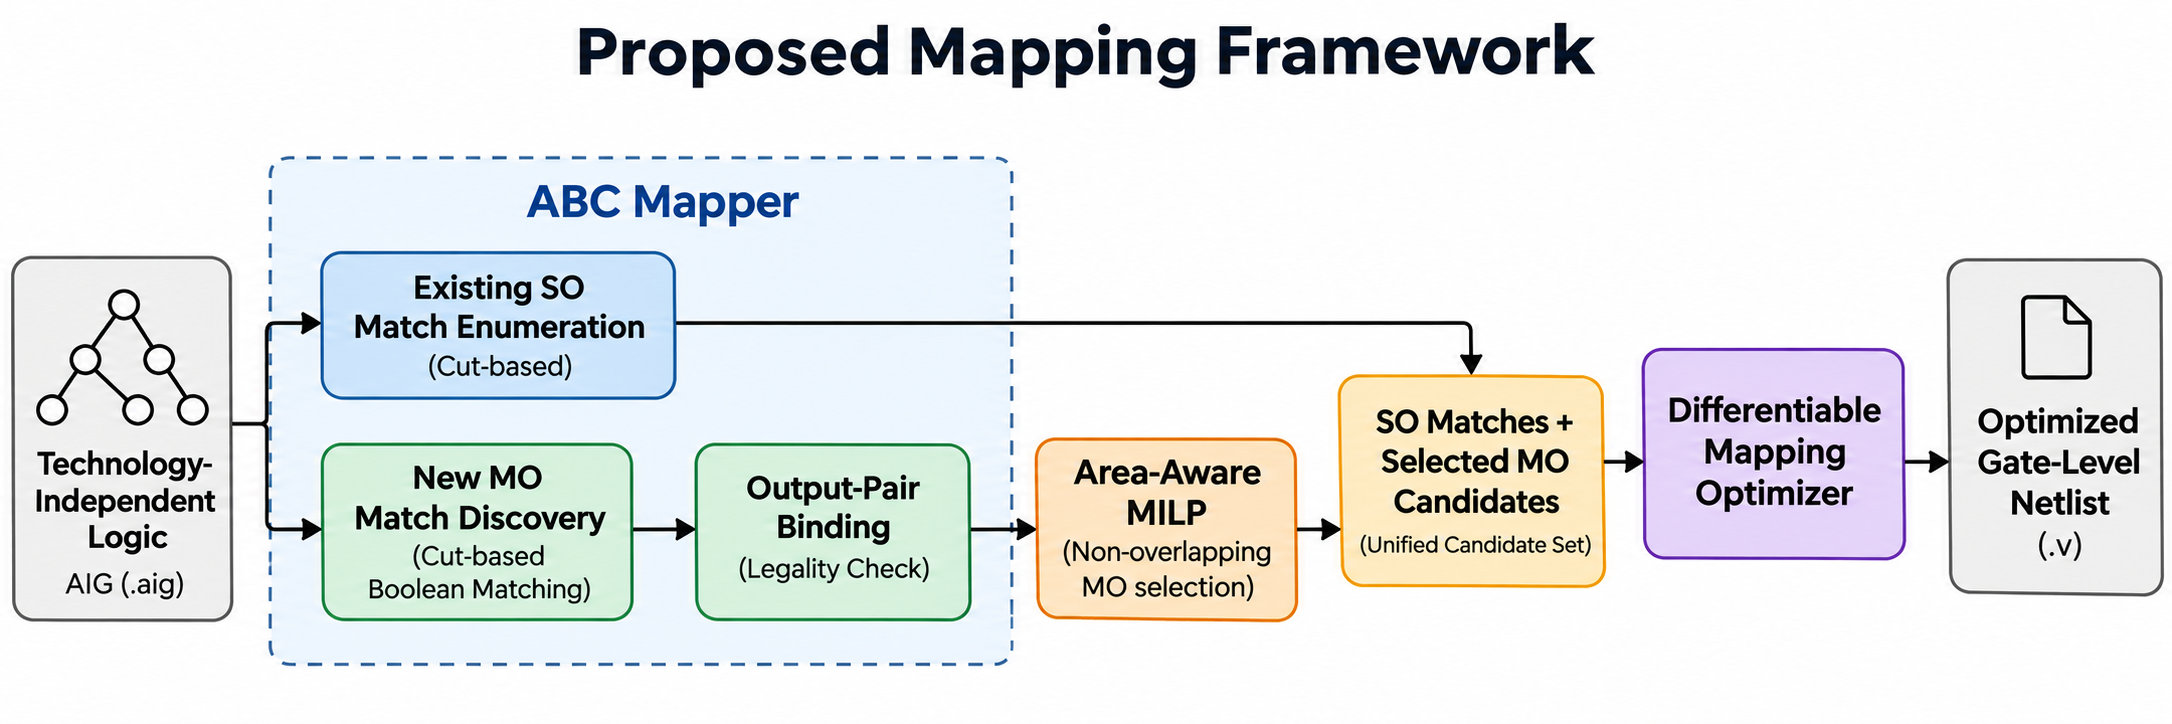
\includegraphics[width=\linewidth,height=4.55cm,keepaspectratio,trim=0 48bp 0 145bp,clip]{mapping-framework.png}
  \end{center}
\end{frame}


% ------------------------------------------------------------------------
% SLIDE 9 / 18 | MO Candidate Discovery in ABC
% ------------------------------------------------------------------------
\renewcommand{\slidenavigation}{\hyperlink{details-index}{\beamerbutton{Details index}}\hspace{.12cm}\hyperlink{detail-legality}{\beamerbutton{Pair legality}}\hspace{.12cm}\hyperlink{detail-witness}{\beamerbutton{SO witness}}}
\renewcommand{\slideposition}{Summary 9 / 18}
\begin{frame}[label=summary-9]{MO Candidate Discovery in ABC}
  \vspace{.02cm}\slidesubtitle{04 / Core Algorithm}\par\vspace{.06cm}
  \takeaway{Identify pairs of logic outputs that can be implemented by a single multi-output standard cell.}
  \vspace{.10cm}
  \begin{columns}[T,onlytextwidth]
    \begin{column}{.32\textwidth}
      \scitem{01 / MO Cut Discovery}{Search for FA/HA-compatible logic cuts independently of SO-oriented pruning.}
    \end{column}
    \begin{column}{.32\textwidth}
      \scitem{02 / Output Pair Matching}{Find SUM and CARRY functions with shared inputs and compatible pin mapping.}
    \end{column}
    \begin{column}{.32\textwidth}
      \scitem{03 / Candidate Validation}{Verify functional and structural legality, then identify the SO logic that the MO cell could replace.}
    \end{column}
  \end{columns}
  \vspace{.12cm}
  \begin{columns}[c,onlytextwidth]
    \begin{column}{.48\textwidth}
      \centering
      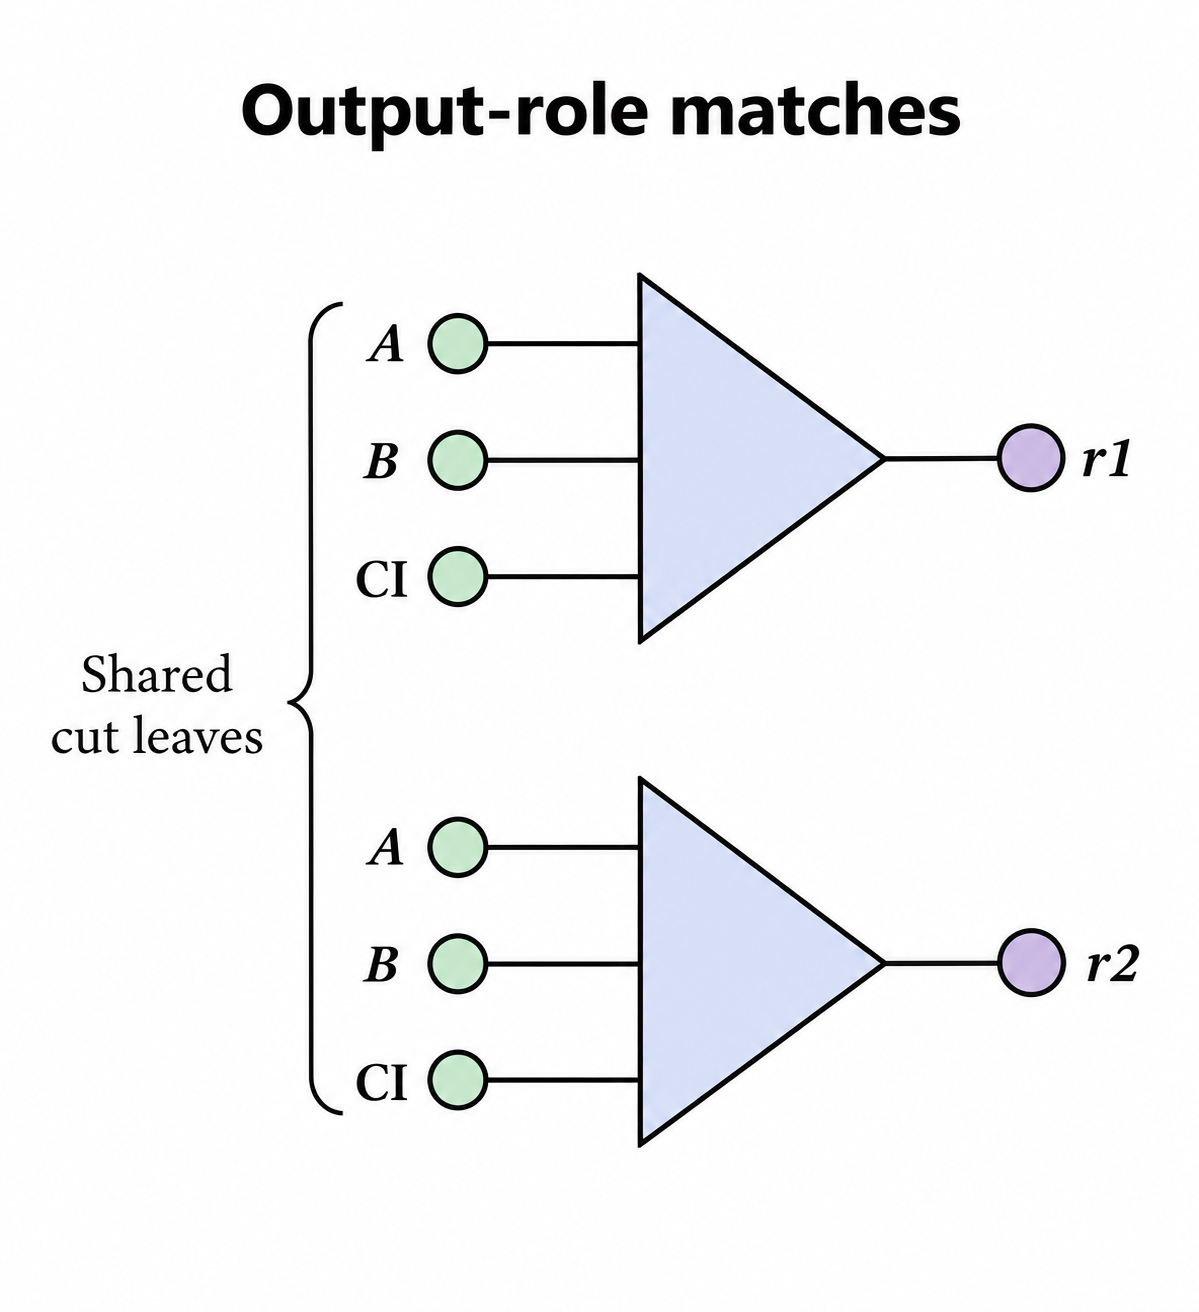
\includegraphics[height=2.95cm,width=\linewidth,keepaspectratio]{shared-cut-leaves.png}
    \end{column}
    \begin{column}{.48\textwidth}
      \centering
      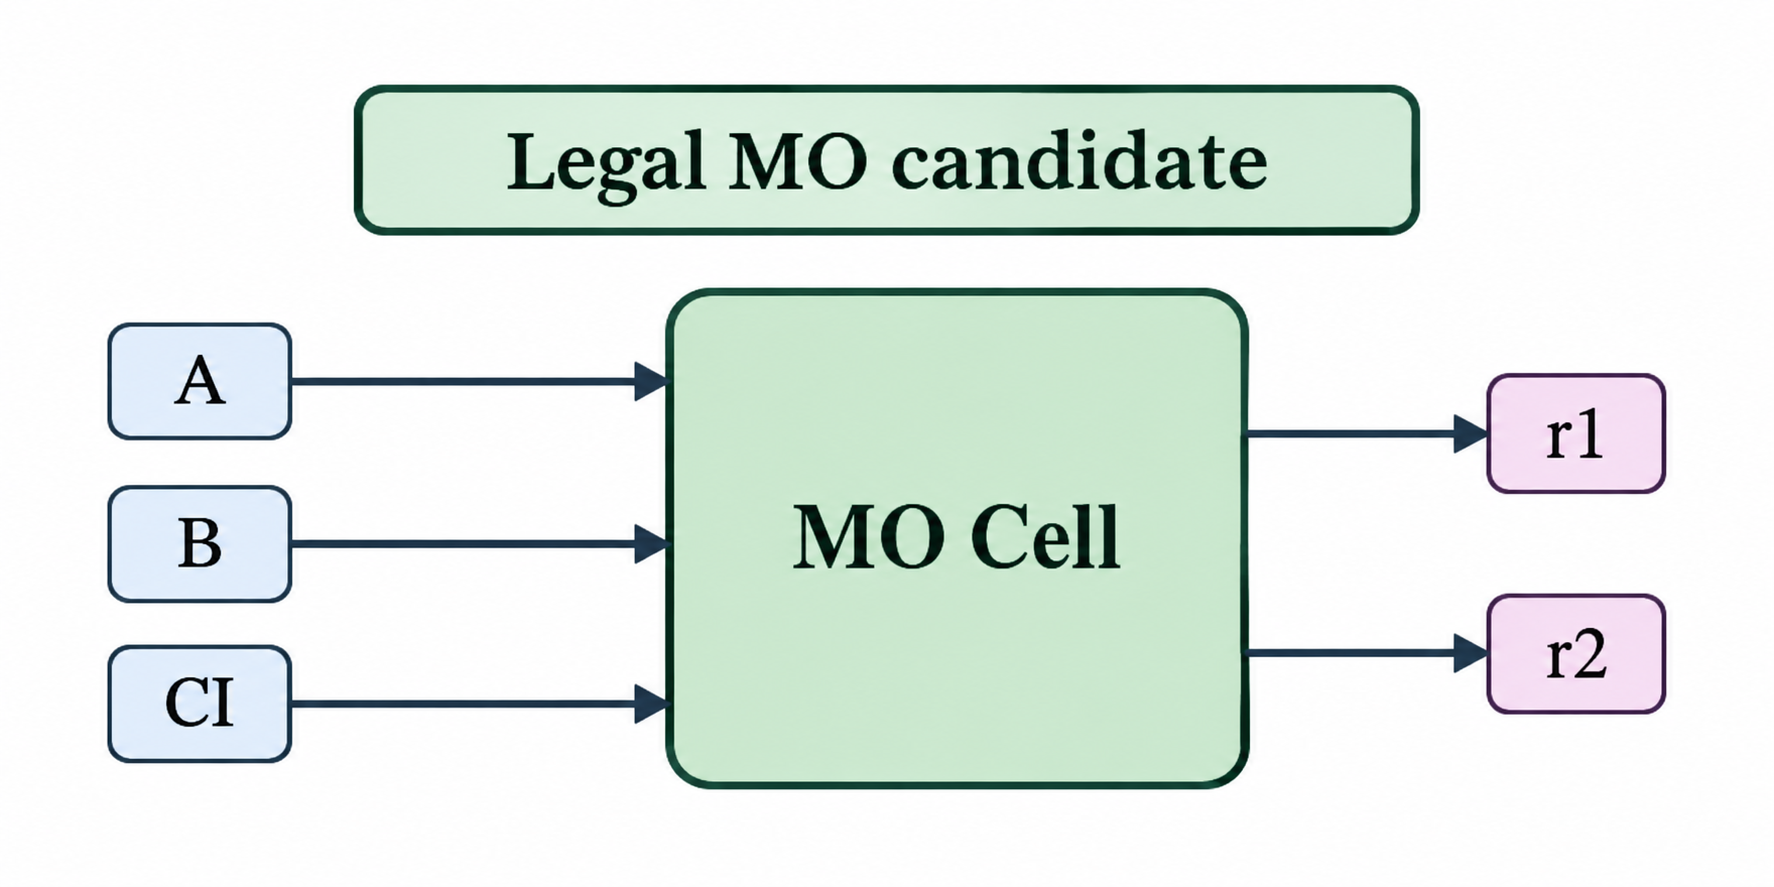
\includegraphics[height=2.95cm,width=\linewidth,keepaspectratio]{legal-mo-candidate.png}
    \end{column}
  \end{columns}
\end{frame}


% ------------------------------------------------------------------------
% SLIDE 10 / 18 | Area-Aware MO Selection (MILP)
% ------------------------------------------------------------------------
\renewcommand{\slidenavigation}{\hyperlink{details-index}{\beamerbutton{Details index}}\hspace{.12cm}\hyperlink{detail-witness}{\beamerbutton{SO witness}}\hspace{.12cm}\hyperlink{detail-verification}{\beamerbutton{Verification}}}
\renewcommand{\slideposition}{Summary 10 / 18}
\begin{frame}[label=summary-10]{Area-Aware MO Selection (MILP)}
  \vspace{.02cm}\slidesubtitle{05 / Global Candidate Selection}\par\vspace{.04cm}
  \takeaway{Maximize estimated area savings subject to non-overlapping MO candidates.}
  \vspace{.06cm}
  \begin{columns}[c,onlytextwidth]
    \begin{column}{.56\textwidth}
      \begin{beamercolorbox}[rounded=true,sep=.08cm,wd=\linewidth]{panelwhite}
      {\normalsize
      \setlength{\abovedisplayskip}{0pt}%
      \setlength{\belowdisplayskip}{0pt}%
      \setlength{\abovedisplayshortskip}{0pt}%
      \setlength{\belowdisplayshortskip}{0pt}%
      \[\boxed{\begin{aligned}
        \max\quad &\sum_{i=1}^{N}\bigl(A_i^{SO}-A_i^{MO}\bigr)x_i\\[1pt]
        \text{s.t.}\quad &\sum_{i=1}^{N} a_{vi}x_i\leq1,\quad\forall v\in\mathcal V\\[1pt]
        &x_i\in\{0,1\},\quad i=1,\ldots,N
      \end{aligned}}\]
      }
      \end{beamercolorbox}
    \end{column}
    \begin{column}{.42\textwidth}
      \centering
      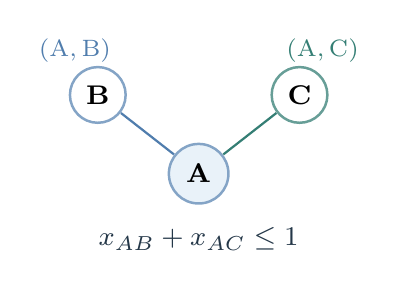
\begin{tikzpicture}[font=\footnotesize,>=Latex,line width=0.9pt,scale=1.22,transform shape]
        \node[circle,draw=AccentBlue!70,fill=SoftBlue,minimum size=0.62cm,inner sep=0pt] (A) at (0,0) {\bfseries A};
        \node[circle,draw=AccentBlue!70,fill=white,minimum size=0.58cm,inner sep=0pt] (B) at (-1.05,0.82) {\bfseries B};
        \node[circle,draw=Accent!75,fill=white,minimum size=0.58cm,inner sep=0pt] (C) at (1.05,0.82) {\bfseries C};
        \draw[AccentBlue,thick] (A) -- (B);
        \draw[Accent,thick] (A) -- (C);
        \node[font=\scriptsize,text=AccentBlue,anchor=east] at (-0.78,1.28) {(A,\,B)};
        \node[font=\scriptsize,text=Accent,anchor=west] at (0.78,1.28) {(A,\,C)};
        \node[font=\footnotesize,text=Ink] at (0,-0.68) {$x_{AB}+x_{AC}\leq 1$};
      \end{tikzpicture}
    \end{column}
  \end{columns}
  \vspace{.02cm}
  \begin{beamercolorbox}[rounded=true,sep=.11cm,wd=\textwidth]{panelblue}
    {\large\bfseries\color{Accent}Notation}\par\vspace{.06cm}
    {\normalsize\color{Ink}
      $x_i$: select MO $i$;\quad $A_i^{SO}$: SO witness area;\quad $A_i^{MO}$: MO cell area;\\[2pt]
      $a_{vi}=1$ iff AIG base node $v$ belongs to MO candidate $i$; otherwise $0$.}
  \end{beamercolorbox}
\end{frame}


% SLIDE 11 / 18 | Mapping Optimizer: SO / BIND Decisions
\renewcommand{\slidenavigation}{\hyperlink{details-index}{\beamerbutton{Details index}}\hspace{.12cm}\hyperlink{detail-verification}{\beamerbutton{Verification}}}
\renewcommand{\slideposition}{Summary 11 / 18}
\begin{frame}[shrink=6,label=summary-11]{Mapping Optimizer: SO / BIND Decisions}
  \vspace{.02cm}\slidesubtitle{06 / Decision Integration}\par\vspace{.06cm}
  \takeaway{MILP pre-selects non-overlapping MO candidates, while the mapping optimizer makes the final SO/BIND decisions.}
  \vspace{.08cm}
  {\centering
    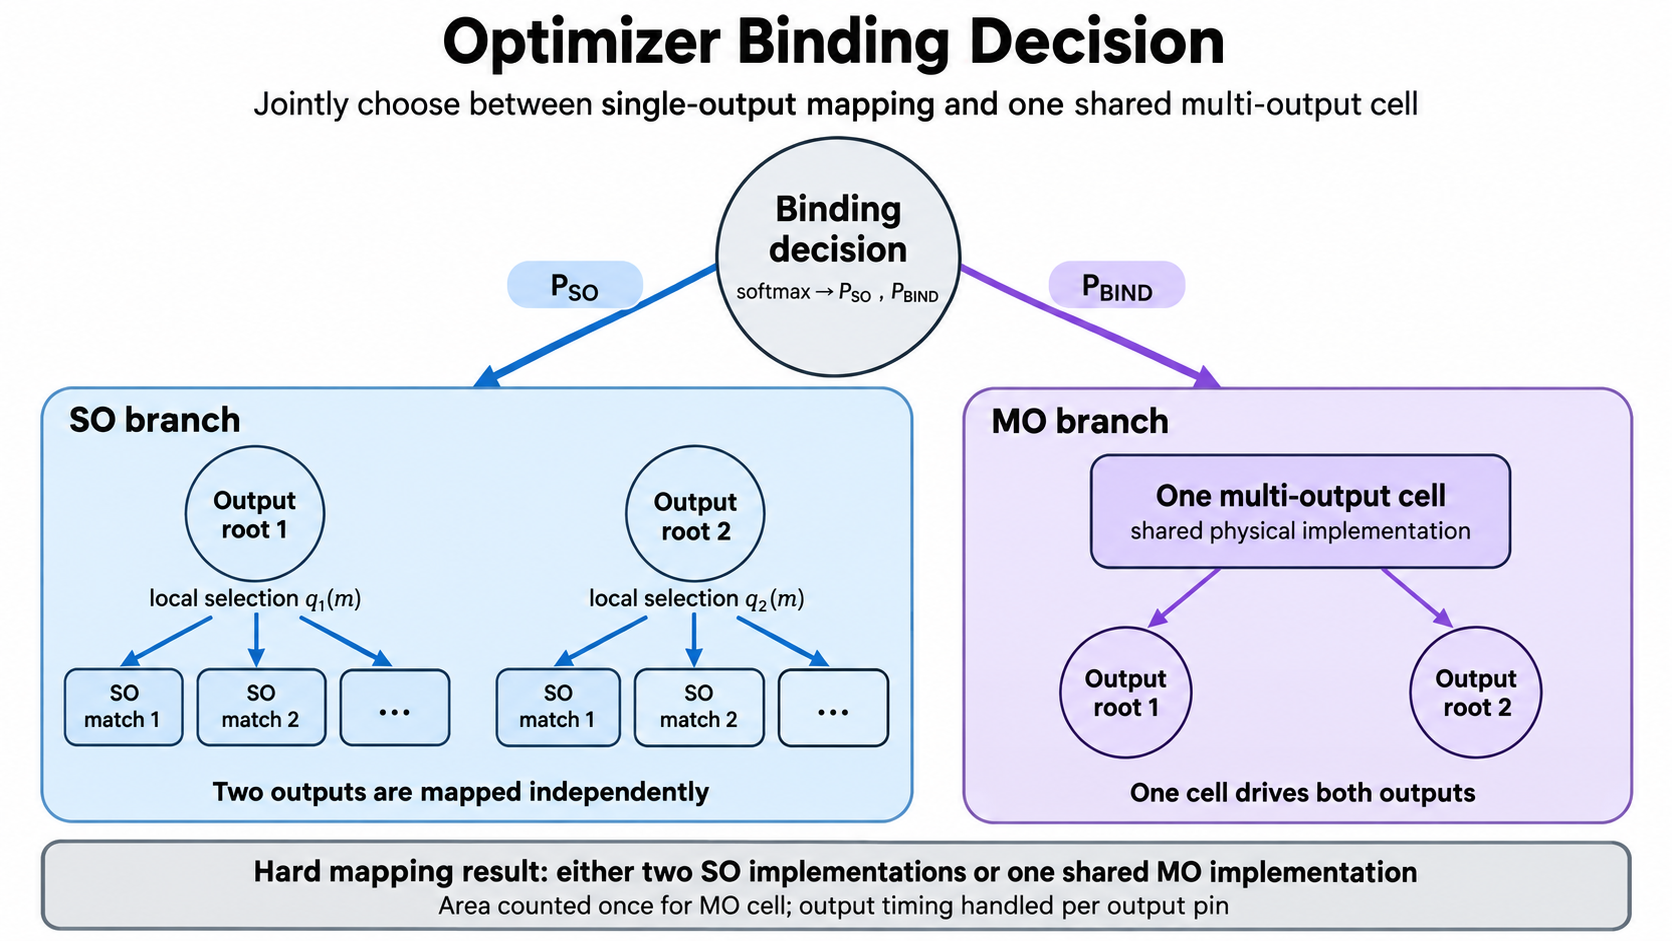
\includegraphics[width=\linewidth,height=5.38cm,keepaspectratio,trim=6bp 112bp 6bp 130bp,clip]{optimizer-binding-decision.png}\par
  }
\end{frame}

% ------------------------------------------------------------------------
% SLIDE 12 / 18 | Normalized ADP results
% Without MILP, ABC = 1.000, SO mode = 0.640, MO mode (FIFO) = 0.627.
% 37.3% is MO mode (FIFO) versus ABC. 2% is that same MO mode versus SO mode.
% 6% below SO mode on the ABC scale: 0.640 x 0.94 = 0.6016, shown as 0.602.
% ------------------------------------------------------------------------
\renewcommand{\slidenavigation}{\hyperlink{details-index}{\beamerbutton{Details index}}\hspace{.12cm}\hyperlink{detail-verification}{\beamerbutton{Verification}}}
\renewcommand{\slideposition}{Summary 12 / 18}
\begin{frame}[label=summary-12]{Normalized ADP Results}
  \slidesubtitle{07 / Current Results}\par\vspace{.06cm}
  \takeaway{Evaluation of four mapping configurations across 30 arithmetic logic circuit benchmarks using the ASAP7 7nm standard-cell library.}
  \vspace{.06cm}
  \begin{columns}[T,onlytextwidth]
    \begin{column}{.54\textwidth}
      {\small\bfseries\color{Ink}GMean Normalized ADP (Area--Delay Product)}\par\vspace{.02cm}
      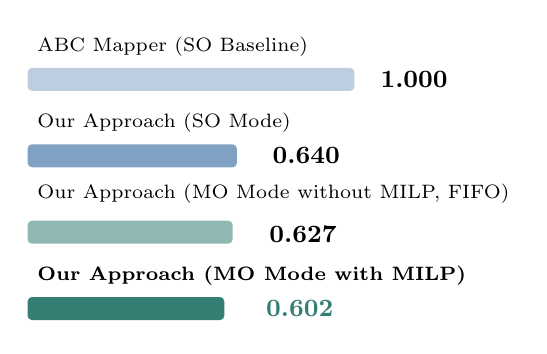
\begin{tikzpicture}[x=4.15cm,y=.97cm]
        \fill[AccentBlue!38,rounded corners=1.5pt] (0,3.00) rectangle (1,3.30);
        \fill[AccentBlue!72,rounded corners=1.5pt] (0,2.00) rectangle (.640,2.30);
        \fill[Accent!55,rounded corners=1.5pt] (0,1.00) rectangle (.627,1.30);
        \fill[Accent,rounded corners=1.5pt] (0,0.00) rectangle (.6016,.30);
        \node[anchor=west,font=\small\bfseries] at (1.05,3.15) {1.000};
        \node[anchor=west,font=\small\bfseries] at (.72,2.15) {0.640};
        \node[anchor=west,font=\small\bfseries] at (.71,1.12) {0.627};
        \node[anchor=west,font=\small\bfseries,text=Accent] at (.70,.15) {0.602};
        \node[anchor=west,font=\scriptsize] at (0,3.58) {ABC Mapper (SO Baseline)};
        \node[anchor=west,font=\scriptsize] at (0,2.58) {Our Approach (SO Mode)};
        \node[anchor=west,font=\scriptsize] at (0,1.66) {Our Approach (MO Mode without MILP, FIFO)};
        \node[anchor=west,font=\scriptsize\bfseries] at (0,.58) {Our Approach (MO Mode with MILP)};
      \end{tikzpicture}\par
      \vspace{.02cm}
      {\scriptsize\color{Muted}FIFO rejects an MO candidate whose root is already used.}
    \end{column}
    \begin{column}{.44\textwidth}
      \begin{beamercolorbox}[rounded=true,sep=.10cm,wd=\linewidth]{block title}
        {\fontsize{18}{20}\selectfont\bfseries\color{Accent}37.3\%}\quad
        {\footnotesize\color{Ink}lower ADP than ABC Mapper}\\[1pt]
        {\scriptsize\color{Muted}Our Approach MO mode (FIFO): 0.627 vs.\ 1.000}
      \end{beamercolorbox}
      \vspace{.06cm}
      \begin{beamercolorbox}[rounded=true,sep=.10cm,wd=\linewidth]{block title}
        {\fontsize{18}{20}\selectfont\bfseries\color{AccentBlue}2\%}\quad
        {\footnotesize\color{Ink}lower ADP than SO mode}\\[1pt]
        {\scriptsize\color{Muted}Our Approach MO mode (FIFO): 0.627 vs.\ 0.640}
      \end{beamercolorbox}
      \vspace{.06cm}
      \begin{beamercolorbox}[rounded=true,sep=.10cm,wd=\linewidth]{block title}
        {\fontsize{18}{20}\selectfont\bfseries\color{Accent}6\%}\quad
        {\footnotesize\color{Ink}lower ADP than SO mode}\\[1pt]
        {\scriptsize\color{Muted}Our Approach MO mode (MILP): 0.602 vs.\ 0.640}
      \end{beamercolorbox}
    \end{column}
  \end{columns}
\end{frame}



% ============================================================
% PROJECT 02 SECTION OPENER | simplified ICCAD 2025 Problem C
% ============================================================
% ------------------------------------------------------------------------
% SLIDE 13 / 18 | Project 02 Opener: ICCAD 2025 CAD Contest Problem C
% ------------------------------------------------------------------------
{\setbeamertemplate{footline}{}
\renewcommand{\slidenavigation}{\hyperlink{details-index}{\beamerbutton{Details index}}}
\renewcommand{\slideposition}{Summary 13 / 18}
\begin{frame}[plain,label=summary-13]
  \vfill
  \smalllabel{Project 02 / ICCAD 2025 CAD Contest / Problem C}\par
  \vspace{.40cm}
  \begin{beamercolorbox}[rounded=true,sep=.25cm,wd=\linewidth]{panelblue}
    {\fontsize{13.6}{17}\selectfont\bfseries\color{Ink}
    \mbox{Incremental Placement Optimization Beyond Detailed Placement}\par}
    \vspace{.14cm}
    {\normalsize\color{Ink}
      Simultaneous Gate Sizing, Buffering, and Cell Relocation\par}
  \end{beamercolorbox}
  \vspace{.80cm}
  \smalllabel{My Proposed Approach}\par
  \vspace{.17cm}
  {\fontsize{18}{23}\selectfont\bfseries\color{Accent}
    STA-Driven Incremental Timing ECO Search\par}
  \vspace{.18cm}
  {\small\color{Muted}
    Use OpenROAD / OpenSTA with policy-controlled ECO moves and global PPA evaluation.\par}
  \vfill
\end{frame}}
% ------------------------------------------------------------------------
% SLIDE 14 / 18 | Multi-Objective Timing ECO Optimization
% ------------------------------------------------------------------------
\renewcommand{\slidenavigation}{\hyperlink{details-index}{\beamerbutton{Details index}}\hspace{.12cm}\hyperlink{detail-targets}{\beamerbutton{STA targets}}\hspace{.12cm}\hyperlink{detail-quality}{\beamerbutton{QoR / budget}}}
\renewcommand{\slideposition}{Summary 14 / 18}
\begin{frame}[label=summary-14]{Multi-Objective Timing ECO Optimization}
  \vspace{.01cm}
  \slidesubtitle{02 / Problem Definition}\par\vspace{.10cm}
  \takeaway{Improve setup TNS toward zero while controlling total power, HPWL, and cell displacement.}
  \vspace{.14cm}

  % ---- Contest objectives: what matters after an ECO repair ----
  \smalllabel{Optimization Objectives}\par\vspace{.08cm}
  \begin{columns}[T,onlytextwidth]
    \begin{column}{.226\textwidth}
      \begin{beamercolorbox}[rounded=true,sep=.14cm,wd=\linewidth]{panelblue}
        {\small\bfseries\color{AccentBlue}01 / Setup TNS}\par\vspace{.11cm}
        {\scriptsize Reduce negative setup\par slack at violating endpoints.}
      \end{beamercolorbox}
    \end{column}
    \begin{column}{.226\textwidth}
      \begin{beamercolorbox}[rounded=true,sep=.14cm,wd=\linewidth]{panelmint}
        {\small\bfseries\color{Accent}02 / Total Power}\par\vspace{.11cm}
        {\scriptsize Avoid excess power\par from ECO changes.}
      \end{beamercolorbox}
    \end{column}
    \begin{column}{.226\textwidth}
      \begin{beamercolorbox}[rounded=true,sep=.14cm,wd=\linewidth]{panellilac}
        {\small\bfseries\color{AccentBlue}03 / HPWL}\par\vspace{.11cm}
        {\scriptsize Control estimated\par wirelength after ECO.}
      \end{beamercolorbox}
    \end{column}
    \begin{column}{.226\textwidth}
      \begin{beamercolorbox}[rounded=true,sep=.14cm,wd=\linewidth]{panelblue}
        {\small\bfseries\color{Accent}04 / Displacement}\par\vspace{.11cm}
        {\scriptsize Limit cell movement\par and keep placement legal.}
      \end{beamercolorbox}
    \end{column}
  \end{columns}

  \vspace{.13cm}
  % ---- Conceptual ECO pipeline, not the proposed branch-search algorithm ----
  \smalllabel{Basic ECO Evaluation Pipeline}\par\vspace{.09cm}
  \centering
  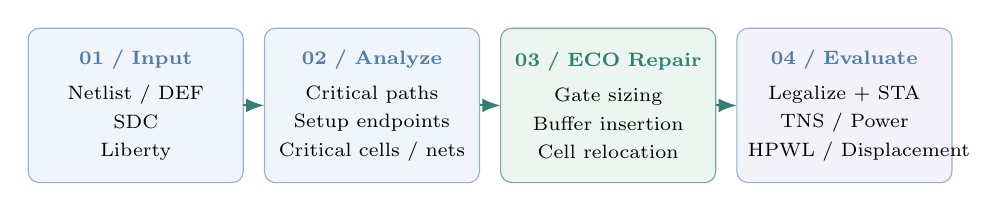
\begin{tikzpicture}[>=Latex,font=\scriptsize]
    \tikzset{
      ecoStage/.style={draw=AccentBlue!60,fill=SoftBlue!74,
        rounded corners=4pt,text width=2.45cm,minimum height=1.96cm,
        inner xsep=4pt,inner ysep=4pt,align=center,outer sep=0pt},
      ecoMint/.style={ecoStage,draw=Accent!68,fill=SoftMint!80},
      ecoLilac/.style={ecoStage,draw=AccentBlue!60,fill=SoftLilac!83}
    }
    \node[ecoStage] (input) at (0,0) {%
      {\bfseries\color{AccentBlue}01 / Input}\\[1.6mm]
      \mbox{Netlist / DEF}\\[.8mm]
      \mbox{SDC}\\[.8mm]
      \mbox{Liberty}};
    \node[ecoStage] (detect) at (3.00,0) {%
      {\bfseries\color{AccentBlue}02 / Analyze}\\[1.6mm]
      \mbox{Critical paths}\\[.8mm]
      \mbox{Setup endpoints}\\[.8mm]
      \mbox{Critical cells / nets}};
    \node[ecoMint] (repair) at (6.00,0) {%
      {\bfseries\color{Accent}03 / ECO Repair}\\[1.6mm]
      \mbox{Gate sizing}\\[.8mm]
      \mbox{Buffer insertion}\\[.8mm]
      \mbox{Cell relocation}};
    \node[ecoLilac] (evaluate) at (9.00,0) {%
      {\bfseries\color{AccentBlue}04 / Evaluate}\\[1.6mm]
      \mbox{Legalize + STA}\\[.8mm]
      \mbox{TNS / Power}\\[.8mm]
      {\fontsize{6.65}{8}\selectfont\mbox{HPWL / Displacement}}};
    \foreach \from/\to in {input/detect,detect/repair,repair/evaluate}{%
      \draw[->,Accent,thick] (\from.east)--(\to.west);}
  \end{tikzpicture}\par
  \vspace{.17cm}
  {\small\bfseries\color{Accent}Key challenge: a timing fix can worsen power or physical cost.\par}
\end{frame}

% ------------------------------------------------------------------------
% SLIDE 15 / 18 | Five Automatic ECO Strategy Candidates
% ------------------------------------------------------------------------
\renewcommand{\slidenavigation}{\hyperlink{details-index}{\beamerbutton{Details index}}\hspace{.12cm}\hyperlink{detail-targets}{\beamerbutton{STA targets}}\hspace{.12cm}\hyperlink{detail-coverage}{\beamerbutton{Endpoint coverage}}\hspace{.12cm}\hyperlink{detail-sequences}{\beamerbutton{ECO sequences}}}
\renewcommand{\slideposition}{Summary 15 / 18}
\begin{frame}[label=summary-15]{Five Automatic ECO Strategy Candidates}
  \vspace{.01cm}
  \slidesubtitle{02 / Candidate Set}\par\vspace{.12cm}
  \takeaway{The candidate is an automatic repair policy and editable region, not a manually chosen cell replacement.}
  \vspace{.37cm}
  \begin{columns}[T,onlytextwidth]
    \begin{column}{.32\textwidth}
      \ecostrategycard{panelblue}{S1 / Global Setup}{Whole design; automatic upsizing and VT selection.}
    \end{column}
    \begin{column}{.32\textwidth}
      \ecostrategycard{panelmint}{S2 / Path-Restricted}{Top-K path cells + nets; localized setup repair.}
    \end{column}
    \begin{column}{.32\textwidth}
      \ecostrategycard{panellilac}{S3 / Overlap-Aware}{Top-I shared cells, nets fixed; sizing / VT repair.}
    \end{column}
  \end{columns}
  \vspace{.34cm}
  \begin{columns}[T,onlytextwidth]
    \begin{column}{.49\textwidth}
      \ecostrategycard{panelmint}{S4 / Local Buffering}{Top-K nets, original cells fixed; buffer insertion and load splitting.}
    \end{column}
    \begin{column}{.49\textwidth}
      \ecostrategycard{panelblue}{S5 / Power Recovery}{Slack-rich cells / wider region; lower-power equivalent cells.}
    \end{column}
  \end{columns}
\end{frame}

% ------------------------------------------------------------------------
% SLIDE 16 / 18 | STA-Guided ECO Search: Best-First Branch List
% ------------------------------------------------------------------------
\renewcommand{\slidenavigation}{\hyperlink{details-index}{\beamerbutton{Details index}}\hspace{.12cm}\hyperlink{detail-quality}{\beamerbutton{QoR / budget}}\hspace{.12cm}\hyperlink{detail-parallel}{\beamerbutton{Parallel workers}}}
\renewcommand{\slideposition}{Summary 16 / 18}
\begin{frame}[label=summary-16]{STA-Guided ECO Search: Best-First Branch List}
  \vspace{.01cm}\slidesubtitle{02 / Heuristic Search Policy}\par\vspace{.07cm}
  \takeaway{No better child this round? Continue from the best unexplored state in the Branch List.}
  \vspace{.13cm}
  \begin{columns}[T,onlytextwidth]
    \begin{column}{.585\textwidth}
      {\small\bfseries\color{Accent}Search Tree Example}\par\vspace{.08cm}
      \centering
      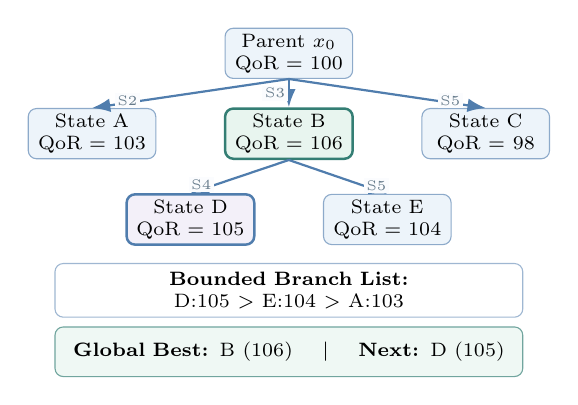
\begin{tikzpicture}[>=Latex,font=\scriptsize]
        \tikzset{
          state/.style={draw=AccentBlue!65,fill=SoftBlue!82,rounded corners=3pt,
            text width=1.48cm,minimum height=.57cm,align=center,inner sep=2pt},
          best/.style={state,draw=Accent,fill=SoftMint!92,line width=.9pt},
          next/.style={state,draw=AccentBlue,fill=SoftLilac!87,line width=.9pt},
          move/.style={font=\tiny,text=Muted,fill=Paper,inner sep=1pt}
        }
        \node[state] (root) at (2.64,0) {Parent $x_0$\\$\mathrm{QoR}=100$};
        \node[state] (a) at (.14,-1.02) {State A\\$\mathrm{QoR}=103$};
        \node[best] (b) at (2.64,-1.02) {State B\\$\mathrm{QoR}=106$};
        \node[state] (c) at (5.14,-1.02) {State C\\$\mathrm{QoR}=98$};
        \draw[->,AccentBlue,thick] (root.south) -- node[move,near end,left]{S2} (a.north);
        \draw[->,AccentBlue,thick] (root.south) -- node[move,midway,left]{S3} (b.north);
        \draw[->,AccentBlue,thick] (root.south) -- node[move,near end,right]{S5} (c.north);
        \node[next] (d) at (1.39,-2.11) {State D\\$\mathrm{QoR}=105$};
        \node[state] (e) at (3.89,-2.11) {State E\\$\mathrm{QoR}=104$};
        \draw[->,AccentBlue,thick] (b.south) -- node[move,near end,left]{S4} (d.north);
        \draw[->,AccentBlue,thick] (b.south) -- node[move,near end,right]{S5} (e.north);
        \node[draw=AccentBlue!55,fill=white,rounded corners=3pt,
          text width=5.73cm,minimum height=.57cm,align=center,inner sep=3pt]
          at (2.64,-3.01) {\textbf{Bounded Branch List:} D:105 $>$ E:104 $>$ A:103};
        \node[draw=Accent!70,fill=SoftMint!65,rounded corners=3pt,
          text width=5.73cm,minimum height=.63cm,align=center,inner sep=3pt]
          at (2.64,-3.79) {\textbf{Global Best:} B (106) \quad $\vert$ \quad
            \textbf{Next:} D (105)};
      \end{tikzpicture}
    \end{column}
    \begin{column}{.395\textwidth}
      {\small\bfseries\color{Accent}Heuristic Search Steps}\par\vspace{.12cm}
      \begin{beamercolorbox}[rounded=true,sep=.15cm,wd=\linewidth]{panelwhite}
        {\small\bfseries\color{Accent}01 / Pop Parent}\par
        {\scriptsize Highest-QoR unexplored state from the \textbf{Branch List}.}\par
        \vspace{.10cm}
        {\small\bfseries\color{Accent}02 / Generate + Evaluate}\par
        {\scriptsize STA-guided ECO moves, legalization, and global QoR score.}\par
        \vspace{.10cm}
        {\small\bfseries\color{Accent}03 / Update States}\par
        {\scriptsize Save improved \textbf{Global Best}; queue legal child states.}\par
        \vspace{.10cm}
        {\small\bfseries\color{Accent}04 / Next Branch}\par
        {\scriptsize Expand best branch, \textbf{even with no new Global Best}.}
      \end{beamercolorbox}
    \end{column}
  \end{columns}
  \vspace{.05cm}
  {\scriptsize\bfseries\color{Accent}A lower-scoring intermediate state may lead to a better ECO sequence later.}\par
\end{frame}

% ------------------------------------------------------------------------
% SLIDE 17 / 18 | QoR Results & Conclusion
% ------------------------------------------------------------------------
\renewcommand{\slidenavigation}{\hyperlink{details-index}{\beamerbutton{Details index}}\hspace{.12cm}\hyperlink{detail-quality}{\beamerbutton{QoR / budget}}}
\renewcommand{\slideposition}{Summary 17 / 18}
\begin{frame}[label=summary-17]{QoR Results \& Conclusion}
  \vspace{.01cm}\slidesubtitle{02 / Earlier ECO Evaluation}\par\vspace{.11cm}
  {\small\color{Muted}Setup-focused timing repair and the resulting power / wirelength trade-off.}\par
  \vspace{.08cm}
  \begin{columns}[T,onlytextwidth]
    \begin{column}{.49\textwidth}
      {\small\bfseries\color{Accent}Setup Timing}\par\vspace{.10cm}
      \begin{beamercolorbox}[rounded=true,sep=.14cm,wd=\linewidth]{panelblue}
        {\fontsize{24}{27}\selectfont\bfseries\color{AccentBlue}16.7\%}\par\vspace{.025cm}
        {\small\bfseries Median Setup TNS Improvement}\par
      \end{beamercolorbox}
      \vspace{.10cm}
      \begin{beamercolorbox}[rounded=true,sep=.14cm,wd=\linewidth]{panellilac}
        {\fontsize{24}{27}\selectfont\bfseries\color{AccentBlue}14.6\%}\par\vspace{.025cm}
        {\small\bfseries Average Setup WNS Improvement}\par
      \end{beamercolorbox}
    \end{column}
    \begin{column}{.49\textwidth}
      {\small\bfseries\color{Accent}Power \& Wirelength}\par\vspace{.10cm}
      \begin{beamercolorbox}[rounded=true,sep=.14cm,wd=\linewidth]{panelmint}
        {\fontsize{24}{27}\selectfont\bfseries\color{Accent}8\%}\par\vspace{.025cm}
        {\small\bfseries Total Power Reduction}\par
      \end{beamercolorbox}
      \vspace{.10cm}
      \begin{beamercolorbox}[rounded=true,sep=.14cm,wd=\linewidth]{panelblue}
        {\fontsize{24}{27}\selectfont\bfseries\color{Ink}+2\%}\par\vspace{.025cm}
        {\small\bfseries HPWL Increase}\par
      \end{beamercolorbox}
    \end{column}
  \end{columns}
  \vspace{.09cm}
  \begin{beamercolorbox}[rounded=true,sep=.13cm,wd=\linewidth]{panelwhite}
    {\small\bfseries\color{Accent}Conclusion}\par\vspace{.025cm}
    {\small\color{Ink}ECO operators can improve setup timing and power while accepting a small wirelength trade-off.}
  \end{beamercolorbox}
  \vspace{.06cm}
\end{frame}

% ------------------------------------------------------------------------
% SLIDE 18 / 18 | Thank You / Questions and Discussion
% ------------------------------------------------------------------------
{\setbeamertemplate{footline}{}
\renewcommand{\slidenavigation}{\hyperlink{details-index}{\beamerbutton{Details index}}}
\renewcommand{\slideposition}{Summary 18 / 18}
\begin{frame}[plain,label=summary-18]
  \centering
  \vfill
  {\fontsize{36}{42}\selectfont\bfseries\color{Ink}THANK YOU}\par
  \vspace{.37cm}
  {\fontsize{19}{24}\selectfont\color{Muted}Questions \& Discussion}\par
  \vfill
\hyperlink{details-index}{\beamergotobutton{Technical details}}\par\vspace{.30cm}
\end{frame}}


% =====================================================================
% Technical details: original full-deck material omitted from the shortlist.
% =====================================================================
\appendix
\renewcommand{\slidenavigation}{\hyperlink{summary-4}{\beamerreturnbutton{Back to project overview}}}
\renewcommand{\slideposition}{Details index}
\begin{frame}[label=details-index]{Technical Details}
  \slidesubtitle{Questions \& Discussion}\par\vspace{.18cm}
  {\small Select a topic. Each detail page links back to the relevant summary slides.}\par
  \vspace{.35cm}
  \begin{columns}[T,onlytextwidth]
\begin{column}{.48\textwidth}
{\normalsize\bfseries\color{Accent}Multi-Output Technology Mapping}\par\vspace{.25cm}
\hyperlink{detail-fifo}{\beamerbutton{D01 / FIFO candidate loss}}\par\vspace{.22cm}
\hyperlink{detail-legality}{\beamerbutton{D02 / Pair legality}}\par\vspace{.22cm}
\hyperlink{detail-witness}{\beamerbutton{D03 / SO witness}}\par\vspace{.22cm}
\hyperlink{detail-verification}{\beamerbutton{D04 / Verification}}\par\vspace{.22cm}
\hyperlink{detail-dc-abc}{\beamerbutton{D10 / DC vs. ABC Synthesis Stages}}\par\vspace{.22cm}
\end{column}
\begin{column}{.48\textwidth}
{\normalsize\bfseries\color{Accent}STA-Driven Timing ECO}\par\vspace{.25cm}
\hyperlink{detail-targets}{\beamerbutton{D05 / STA targets}}\par\vspace{.22cm}
\hyperlink{detail-coverage}{\beamerbutton{D06 / Endpoint coverage}}\par\vspace{.22cm}
\hyperlink{detail-sequences}{\beamerbutton{D07 / ECO sequences}}\par\vspace{.22cm}
\hyperlink{detail-quality}{\beamerbutton{D08 / QoR / budget}}\par\vspace{.22cm}
\hyperlink{detail-parallel}{\beamerbutton{D09 / Parallel workers}}\par\vspace{.22cm}
\end{column}
\end{columns}\end{frame}

% DETAIL 01 / 10 | File-order candidate loss
\renewcommand{\slidenavigation}{\hyperlink{details-index}{\beamerbutton{Details index}}\hspace{.12cm}\hyperlink{summary-10}{\beamerreturnbutton{Summary 10}}\hspace{.12cm}\hyperlink{summary-11}{\beamerreturnbutton{Summary 11}}}
\renewcommand{\slideposition}{Detail 1 / 10}
\begin{frame}[shrink=8,label=detail-fifo]{Baseline: File-Order Candidate Loss}
  \vspace{.02cm}\slidesubtitle{08 / Motivation for MILP}\par\vspace{.08cm}
  \takeaway{File-order greedy filtering ignores estimated area benefits of conflicting MO candidates.}
  \vspace{.17cm}
  \begin{columns}[T,onlytextwidth]
    \begin{column}{.319\textwidth}\statcard{41,476}{Original MO candidate BIND records}\end{column}
    \begin{column}{.319\textwidth}\statcard{7,024}{FIFO retained (offline simulation)}\end{column}
    \begin{column}{.319\textwidth}\statcard{16.9\%}{Overall retention rate}\end{column}
  \end{columns}
  \vspace{.07cm}
  \begin{center}
  \footnotesize
\begin{tabular}{@{}lrrrr@{}}
\toprule
\textbf{Design} & \textbf{Original MO} & \textbf{FIFO Retained} & \textbf{Dropped} & \textbf{Retention} \\
\midrule
EPFL hyp & 25,440 & 4,180 & 21,260 & 16.4\% \\
EPFL square & 3,658 & 544 & 3,114 & 14.9\% \\
EPFL log2 & 2,798 & 400 & 2,398 & 14.3\% \\
EPFL multiplier & 2,190 & 349 & 1,841 & 15.9\% \\
EPFL voter & 632 & 106 & 526 & 16.8\% \\
ISCAS c6288 & 258 & 37 & 221 & 14.3\% \\
ISCAS c7552 & 102 & 11 & 91 & 10.8\% \\
EPFL adder & 6 & 1 & 5 & 16.7\% \\
\textbf{All 364 designs} & \textbf{41,476} & \textbf{7,024} & \textbf{34,452} & \textbf{16.9\%} \\
\bottomrule
\end{tabular}
  \end{center}
  \vspace{-0.02cm}
  {\tiny\color{Muted}Source: MO-candidate census, 364 benchmark entries; simulated first-fit retention, not mapping-optimizer QoR.}
\end{frame}

% DETAIL 02 / 10 | Pair legality (original full-deck slide 9)
\renewcommand{\slidenavigation}{\hyperlink{details-index}{\beamerbutton{Details index}}\hspace{.12cm}\hyperlink{summary-9}{\beamerreturnbutton{Summary 9}}}
\renewcommand{\slideposition}{Detail 2 / 10}
\begin{frame}[label=detail-legality]{MO Pair Matching \& Structural Legality}
  \vspace{.02cm}\slidesubtitle{05 / Candidate Validation}\par\vspace{.06cm}
  \takeaway{Individual legality is checked here; the MILP selects a conflict-free set.}
  \vspace{.04cm}
  \begin{columns}[T,onlytextwidth]
    \begin{column}{.318\textwidth}
      \smallpanel{panelblue}{Boolean Matching}{CON and SN roots match the cell's SUM and CARRY truth tables.}
    \end{column}
    \begin{column}{.318\textwidth}
      \smallpanel{panelmint}{Pin Compatibility}{Shared input support, with a compatible pin permutation and polarity.}
    \end{column}
    \begin{column}{.318\textwidth}
      \smallpanel{panellilac}{Structural Legality}{Distinct roots. Reject direct-dangling and TFI or cycle conflicts.}
    \end{column}
  \end{columns}
  \vspace{.10cm}
  \begin{columns}[T,onlytextwidth]
    \begin{column}{.56\textwidth}
      \centering
      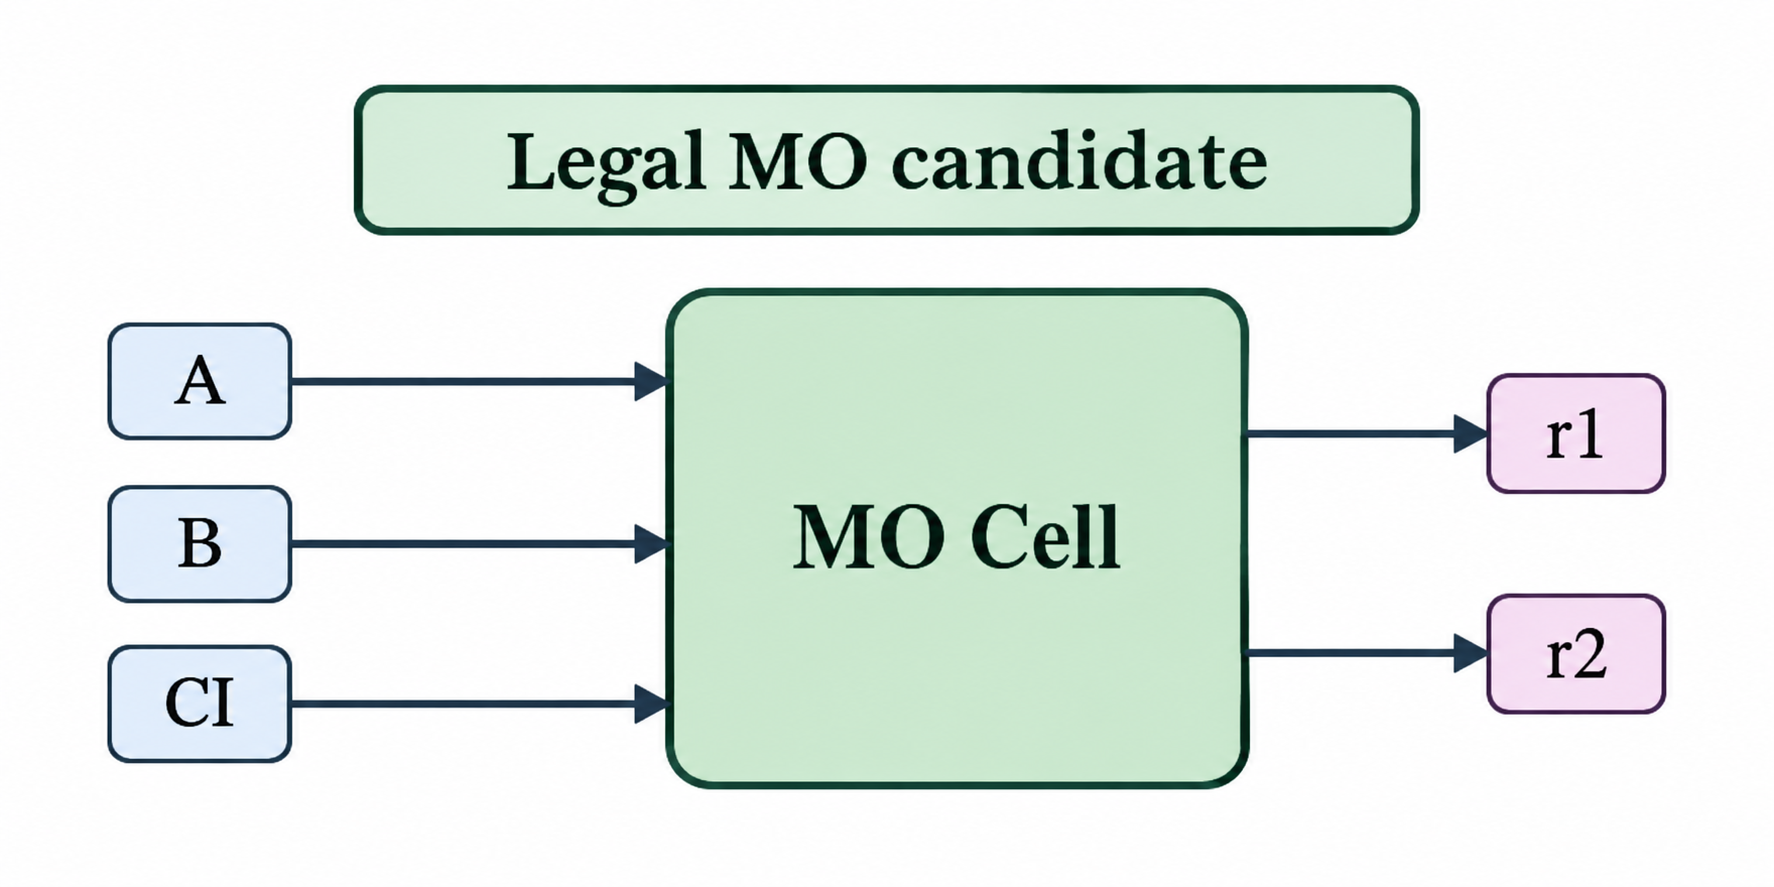
\includegraphics[width=\linewidth,height=2.05cm,keepaspectratio]{legal-mo-candidate.png}
    \end{column}
    \begin{column}{.42\textwidth}
      {\small\bfseries\color{Accent}Individual MO Candidate Legality}\par\vspace{.04cm}
      {\scriptsize Function, pins, structure, and the SO replacement witness are checked for one candidate.}
      \vspace{.12cm}
      {\small\bfseries\color{Accent}Global Conflict-Free MO Selection}\par\vspace{.04cm}
      {\scriptsize Overlapping candidates are resolved by the area-aware MILP, not by this check.}
    \end{column}
  \end{columns}
  \vspace{.02cm}
  {\scriptsize\color{Muted}CON/SN name the two output roles. A legal record stores BIND, ROOTS, FANINS, and REPLACE\_ROOTS.}
\end{frame}

% DETAIL 03 / 10 | SO witness (original full-deck slide 10)
\renewcommand{\slidenavigation}{\hyperlink{details-index}{\beamerbutton{Details index}}\hspace{.12cm}\hyperlink{summary-9}{\beamerreturnbutton{Summary 9}}\hspace{.12cm}\hyperlink{summary-10}{\beamerreturnbutton{Summary 10}}}
\renewcommand{\slideposition}{Detail 3 / 10}
\begin{frame}[label=detail-witness]{SO Witness: Replacing Multiple SO Cells}
  \slidesubtitle{06 / Replacement Semantics}\par\vspace{.10cm}
  \takeaway{An MO candidate replaces a multi-level SO subcover with two output roots.}
  \vspace{.12cm}
  \begin{columns}[T,onlytextwidth]
    \begin{column}{.49\textwidth}
      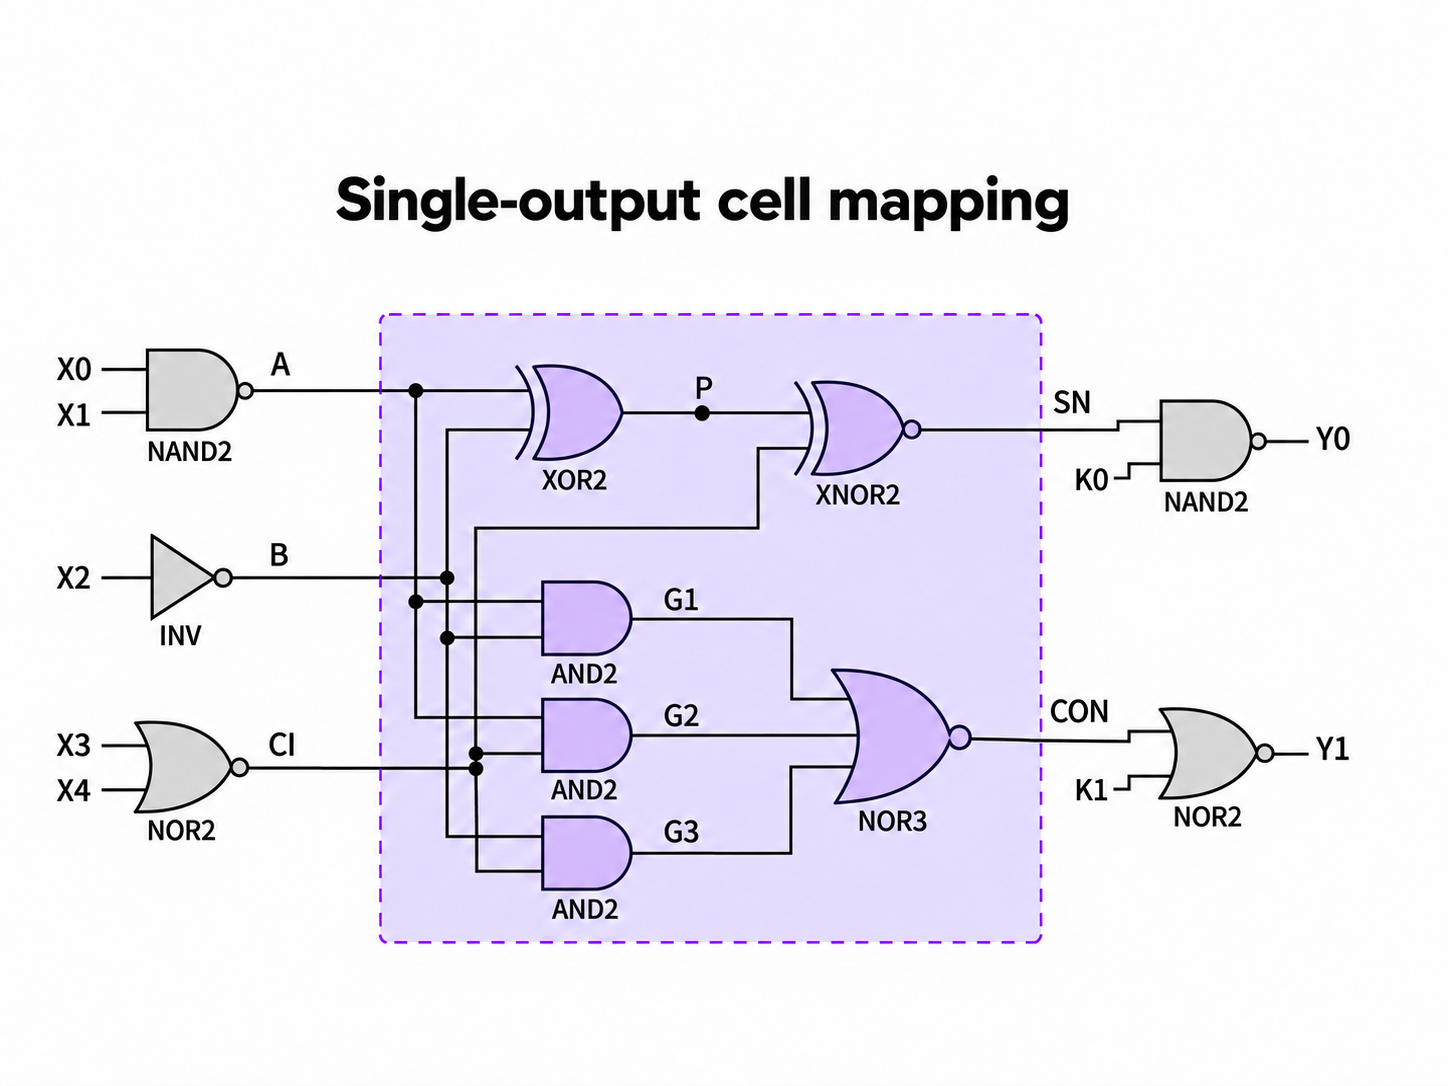
\includegraphics[width=\linewidth,height=3.45cm,keepaspectratio,trim=0 105bp 0 250bp,clip]{single-output-cell-mapping.png}
    \end{column}
    \begin{column}{.49\textwidth}
      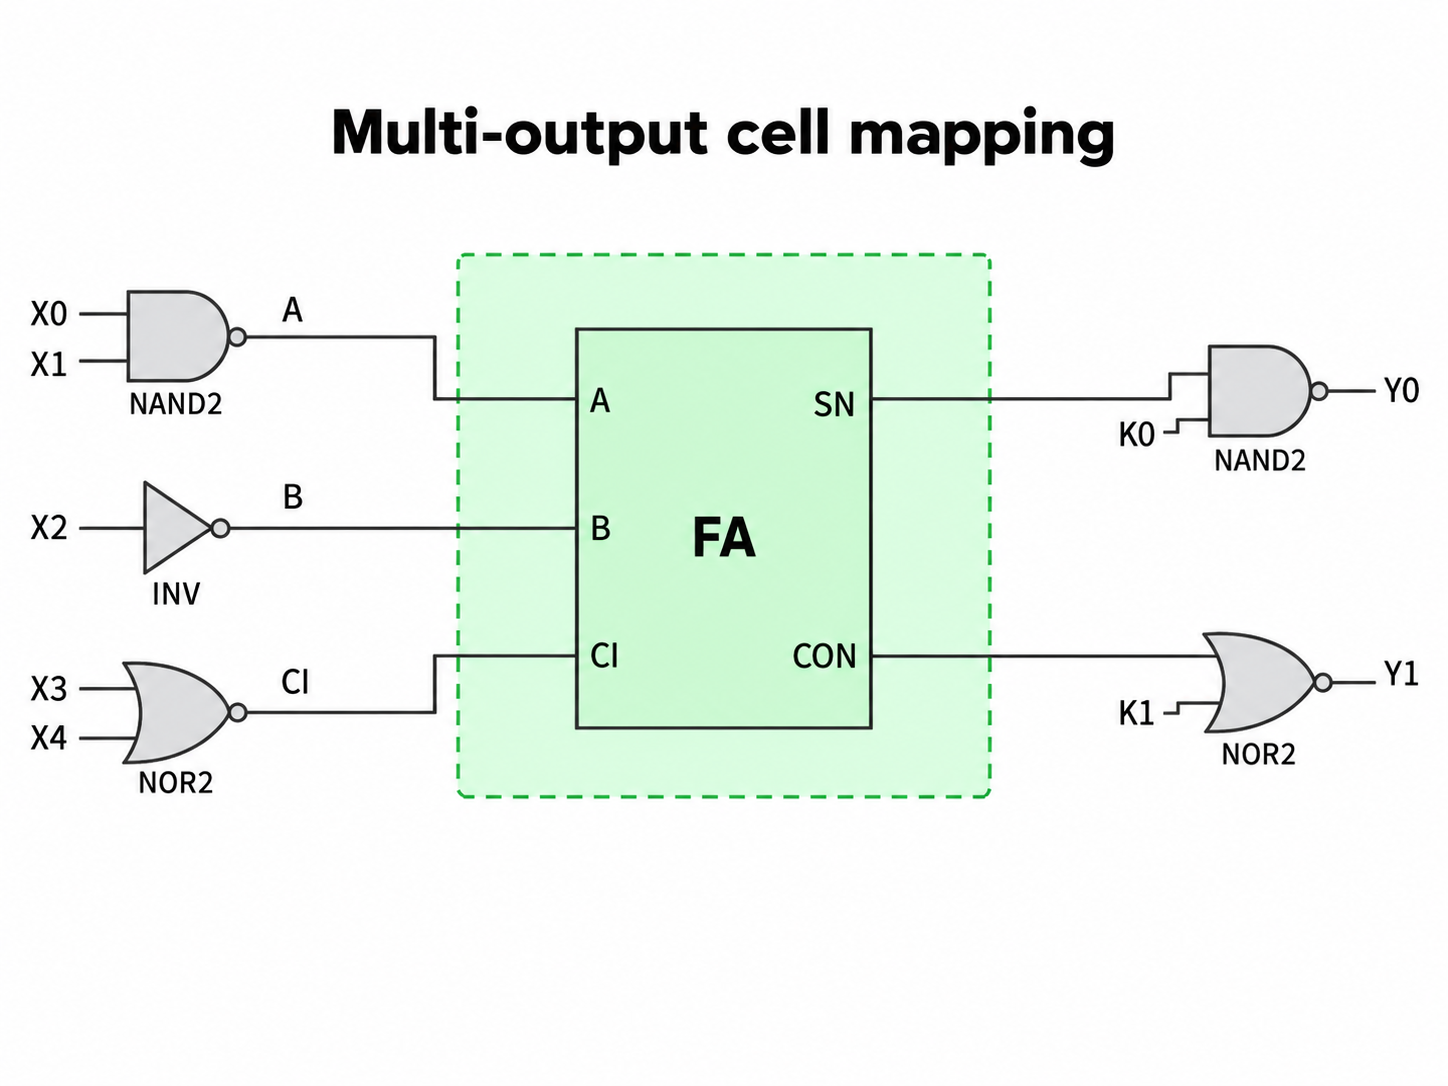
\includegraphics[width=\linewidth,height=3.45cm,keepaspectratio,trim=0 180bp 0 175bp,clip]{multi-output-cell-mapping.png}
    \end{column}
  \end{columns}
  \vspace{.13cm}
  {\small Trace the SO witness to the common MO input boundary. Record participating nodes as
  \texttt{REPLACE\_ROOTS}; preserve any internal node still demanded externally.}\par
  \vspace{.10cm}
  {\scriptsize\color{Muted}The SO witness need not equal ABC's final selected SO cover.}
\end{frame}

% DETAIL 04 / 10 | Verification (original full-deck slide 14)
\renewcommand{\slidenavigation}{\hyperlink{details-index}{\beamerbutton{Details index}}\hspace{.12cm}\hyperlink{summary-10}{\beamerreturnbutton{Summary 10}}\hspace{.12cm}\hyperlink{summary-12}{\beamerreturnbutton{Summary 12}}}
\renewcommand{\slideposition}{Detail 4 / 10}
\begin{frame}[shrink=8,label=detail-verification]{Python + HiGHS: Verification Pipeline}
  \vspace{.02cm}\slidesubtitle{10 / Reproducible Evaluation}\par\vspace{.08cm}
  \takeaway{Separate MILP pre-selection quality from the mapping optimizer's final mapped area.}
  \vspace{.18cm}
  \begin{center}
  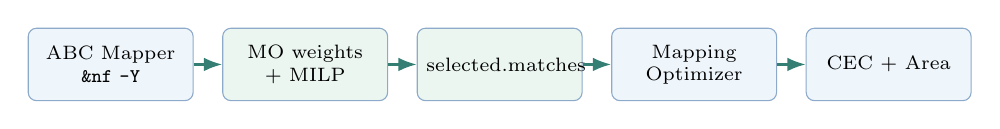
\begin{tikzpicture}[>=Latex,font=\scriptsize]
    \tikzset{b/.style={draw=AccentBlue!65,fill=SoftBlue!72,rounded corners=3pt,
      text width=1.86cm,minimum height=.92cm,align=center}}
    \node[b](a) at (0,0) {ABC Mapper\\ \texttt{\&nf -Y}};
    \node[b,fill=SoftMint!80](b) at (2.47,0) {MO weights + MILP};
    \node[b,fill=SoftMint!80](c) at (4.94,0) {selected.matches};
    \node[b](d) at (7.41,0) {Mapping Optimizer};
    \node[b](e) at (9.88,0) {CEC + Area};
    \foreach \u/\v in {a/b,b/c,c/d,d/e}{\draw[->,Accent,thick](\u.east)--(\v.west);}
  \end{tikzpicture}\par
  \vspace{.04cm}
  {\scriptsize\color{Muted}The MILP filters MO candidates. SO matches from the ABC Mapper stay available to the optimizer.}
  \end{center}
  \vspace{.14cm}
  \smallpanel{panelmint}{Implementation}{Python + HiGHS (\texttt{highspy}); emit selected.matches.}
  \vspace{.12cm}
  \begin{columns}[T,onlytextwidth]
    \begin{column}{.48\textwidth}
      \softpanel{panelblue}{Correctness Checks}{Gate A: unchanged ABC Mapper results\\ Gate B: individual MO legality\\ Gate C: optimizer materialization + CEC}
    \end{column}
    \begin{column}{.48\textwidth}
      \softpanel{panelmint}{Experimental Comparison}{SO-only vs FIFO vs MILP-selected MO; same AIG, library, optimizer settings, and seed.}
    \end{column}
  \end{columns}
  \vspace{.12cm}
  % The old results graphic reported 2\% extra ADP reduction and is not reusable.
  % Summary slide 12 already states the current 6\% ADP reduction versus SO mode.
  % This slot is for a later SO-only / FIFO / MILP comparison if that chart is drawn.
  \figurespace{0.78cm}{ADP and runtime chart}{SO-only, FIFO, and MILP-selected MO, under the same settings.}
\end{frame}

% DETAIL 05 / 10 | STA targets (original full-deck slide 19)
\renewcommand{\slidenavigation}{\hyperlink{details-index}{\beamerbutton{Details index}}\hspace{.12cm}\hyperlink{summary-14}{\beamerreturnbutton{Summary 14}}\hspace{.12cm}\hyperlink{summary-15}{\beamerreturnbutton{Summary 15}}}
\renewcommand{\slideposition}{Detail 5 / 10}
\begin{frame}[shrink=10,label=detail-targets]{Timing-Driven Target Extraction}
  \vspace{.01cm}\slidesubtitle{02 / STA Analysis}\par\vspace{.08cm}
  \takeaway{Derive editable cells and nets from setup-violating paths and distinct endpoints.}
  \vspace{.18cm}
  \begin{columns}[T,onlytextwidth]
    \begin{column}{.52\textwidth}
      \begin{beamercolorbox}[rounded=true,sep=.18cm,wd=\linewidth]{panelwhite}
        {\ttfamily\scriptsize
        report\_checks -path\_delay max \\
        \hspace{7mm}-group\_count 200 \\
        \hspace{7mm}-endpoint\_count 3 \\
        \hspace{7mm}-slack\_max 0}
      \end{beamercolorbox}
      \vspace{.16cm}
      \smallpanel{panelblue}{STA Report Scope}{Setup paths may be PI$\rightarrow$FF, FF$\rightarrow$FF, FF$\rightarrow$PO, or PI$\rightarrow$PO, depending on constraints.}
    \end{column}
    \begin{column}{.44\textwidth}
      \scitem{1 / Extract}{Record endpoint, slack, path instances and nets.}
      \vspace{.14cm}
      \scitem{2 / Deduplicate}{Do not count the same violating endpoint repeatedly.}
      \vspace{.14cm}
      \scitem{3 / Prioritize}{Rank shared cells, critical nets, and candidate repair regions.}
    \end{column}
  \end{columns}
  \vspace{.26cm}
  \begin{beamercolorbox}[rounded=true,sep=.15cm,wd=\linewidth]{panelmint}
    {\small\bfseries\color{Accent}The STA report chooses where to search; OpenROAD performs the actual repair operation.}
  \end{beamercolorbox}
\end{frame}

% DETAIL 06 / 10 | Endpoint coverage (original full-deck slide 20)
\renewcommand{\slidenavigation}{\hyperlink{details-index}{\beamerbutton{Details index}}\hspace{.12cm}\hyperlink{summary-15}{\beamerreturnbutton{Summary 15}}}
\renewcommand{\slideposition}{Detail 6 / 10}
\begin{frame}[shrink=5,label=detail-coverage]{Slack-Weighted Endpoint Coverage}
  \vspace{.01cm}\slidesubtitle{02 / Ranking Heuristic}\par\vspace{.08cm}
  \takeaway{Prioritize shared cells by distinct endpoint coverage and violation severity.}
  \vspace{.20cm}
  \begin{columns}[T,onlytextwidth]
    \begin{column}{.56\textwidth}
      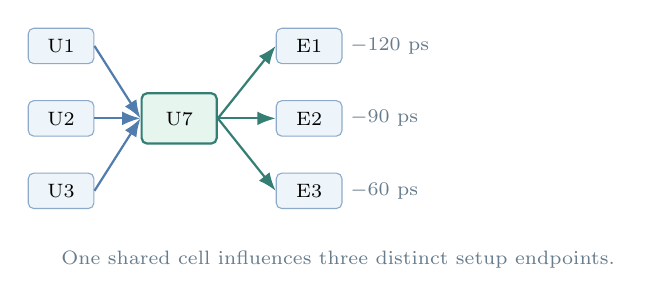
\begin{tikzpicture}[>=Latex,font=\scriptsize]
        \tikzset{b/.style={draw=AccentBlue!65,fill=SoftBlue!80,rounded corners=2pt,text width=.60cm,minimum height=.45cm,align=center},
                  h/.style={b,draw=Accent,fill=SoftMint!95,thick,text width=.72cm,minimum height=.64cm}}
        \node[b](u1)at(0,0){U1};
        \node[b](u2)at(0,-.92){U2};
        \node[b](u3)at(0,-1.84){U3};
        \node[h](shared)at(1.50,-.92){U7};
        \node[b](e1)at(3.15,0){E1};
        \node[b](e2)at(3.15,-.92){E2};
        \node[b](e3)at(3.15,-1.84){E3};
        \foreach \n in {u1,u2,u3}{\draw[->,AccentBlue,thick](\n.east)--(shared.west);}
        \foreach \n in {e1,e2,e3}{\draw[->,Accent,thick](shared.east)--(\n.west);}
        \node[anchor=west,text=Muted]at(3.55,0){$-120$ ps};
        \node[anchor=west,text=Muted]at(3.55,-.92){$-90$ ps};
        \node[anchor=west,text=Muted]at(3.55,-1.84){$-60$ ps};
        \node[anchor=west,align=left,text=Muted] at (-.12,-2.72) {One shared cell influences three distinct setup endpoints.};
      \end{tikzpicture}
    \end{column}
    \begin{column}{.40\textwidth}
      \smallpanel{panelmint}{Distinct Endpoint Coverage}{$Coverage(c)=|E(c)|$\par Each endpoint is counted only once.}
      \vspace{.16cm}
      \smallpanel{panelblue}{Slack-Weighted Priority}{$Priority(c)=\sum_{e\in E(c)}\max(0,-slack_e)$}
    \end{column}
  \end{columns}
  \vspace{.26cm}
  \begin{beamercolorbox}[rounded=true,sep=.17cm,wd=\linewidth]{panelwhite}
    {\small\bfseries\color{Accent}This priority guides search; the real $\Delta TNS$ still requires global STA after ECO.}
  \end{beamercolorbox}
\end{frame}

% DETAIL 07 / 10 | ECO sequences (original full-deck slide 21)
\renewcommand{\slidenavigation}{\hyperlink{details-index}{\beamerbutton{Details index}}\hspace{.12cm}\hyperlink{summary-15}{\beamerreturnbutton{Summary 15}}}
\renewcommand{\slideposition}{Detail 7 / 10}
\begin{frame}[shrink=6,label=detail-sequences]{Sequential ECO Strategy Combinations}
  \vspace{.01cm}\slidesubtitle{02 / Multi-Step Candidates}\par\vspace{.08cm}
  \takeaway{Build a candidate by chaining compatible automatic repairs from a saved checkpoint.}
  \vspace{.17cm}
  \begin{columns}[T,onlytextwidth]
    \begin{column}{.52\textwidth}
      \smallpanel{panelblue}{S3 $\rightarrow$ S5}{Repair shared timing-critical cells, then attempt power recovery if slack permits.}
      \vspace{.14cm}
      \smallpanel{panelmint}{S4 $\rightarrow$ S3}{Buffer selected critical nets, then re-target the remaining critical cells.}
      \vspace{.14cm}
      \smallpanel{panellilac}{S3 $\rightarrow$ S4}{Size critical cells first, then address residual net-delay bottlenecks.}
    \end{column}
    \begin{column}{.44\textwidth}
      \begin{beamercolorbox}[rounded=true,sep=.20cm,wd=\linewidth]{panelwhite}
        {\scriptsize\bfseries\color{Accent}Candidate Execution}\par\vspace{.13cm}
        {\small Parent checkpoint}\par\vspace{.10cm}
        {\scriptsize\color{Accent}$\downarrow$}\par\vspace{.08cm}
        {\small Automatic repair pass 1}\par\vspace{.10cm}
        {\scriptsize\color{Accent}$\downarrow$}\par\vspace{.08cm}
        {\small Optional repair pass 2}\par\vspace{.10cm}
        {\scriptsize\color{Accent}$\downarrow$}\par\vspace{.08cm}
        {\small Legalize + re-evaluate global QoR}
      \end{beamercolorbox}
    \end{column}
  \end{columns}
  \vspace{.18cm}
  {\small\bfseries\color{Accent}Operator order matters: buffering changes load; sizing changes driver strength.}
\end{frame}

% DETAIL 08 / 10 | QoR / budget (original full-deck slide 22)
\renewcommand{\slidenavigation}{\hyperlink{details-index}{\beamerbutton{Details index}}\hspace{.12cm}\hyperlink{summary-14}{\beamerreturnbutton{Summary 14}}\hspace{.12cm}\hyperlink{summary-16}{\beamerreturnbutton{Summary 16}}\hspace{.12cm}\hyperlink{summary-17}{\beamerreturnbutton{Summary 17}}}
\renewcommand{\slideposition}{Detail 8 / 10}
\begin{frame}[shrink=9,label=detail-quality]{Checkpoint Quality and Runtime Budget}
  \vspace{.01cm}\slidesubtitle{02 / Branch List Ranking}\par\vspace{.08cm}
  \takeaway{Rank legal ECO checkpoints with consistent global QoR references, under one runtime budget.}
  \vspace{.11cm}
  \smalllabel{Illustrative Internal Ranking Score}\par\vspace{.07cm}
  \begin{beamercolorbox}[rounded=true,sep=.12cm,wd=\linewidth]{panelwhite}
  {\small
  \[\boxed{Q(x) = w_T\,g_T(x) + w_P\,g_P(x) - w_H\,p_H(x)}\]
  \vspace{-.08cm}
  \[g_T=\frac{|TNS_0|-|TNS_x|}{\max(|TNS_0|,\epsilon)},\quad
    g_P=\frac{P_0-P_x}{P_0},\quad
    p_H=\frac{H_x-H_0}{H_0}\]
  }
  \end{beamercolorbox}
  \vspace{.15cm}
  \begin{columns}[T,onlytextwidth]
    \begin{column}{.48\textwidth}
      \smallpanel{panelblue}{Quality-Based Search}{Use the same baseline and weights when evaluating different branches; reject illegal or failed ECO states.}
    \end{column}
    \begin{column}{.48\textwidth}
      \smallpanel{panelmint}{Runtime-Aware Execution}{Batch processing consumes wall-clock time once; stop when the global execution budget is exhausted.}
    \end{column}
  \end{columns}
  \vspace{.14cm}
  {\scriptsize\color{Muted}$TNS$: setup total negative slack; $P$: total power; $H$: HPWL. Weights define a search heuristic, not an official contest score.}
\end{frame}

% DETAIL 09 / 10 | Parallel workers (original full-deck slide 24)
\renewcommand{\slidenavigation}{\hyperlink{details-index}{\beamerbutton{Details index}}\hspace{.12cm}\hyperlink{summary-16}{\beamerreturnbutton{Summary 16}}}
\renewcommand{\slideposition}{Detail 9 / 10}
\begin{frame}[shrink=8,label=detail-parallel]{Parallel Candidate Evaluation with OpenROAD}
  \vspace{.01cm}\slidesubtitle{02 / Execution Architecture}\par\vspace{.08cm}
  \takeaway{Independent workers run candidate ECO sequences from a selected Branch List checkpoint.}
  \vspace{.16cm}
  \begin{center}
  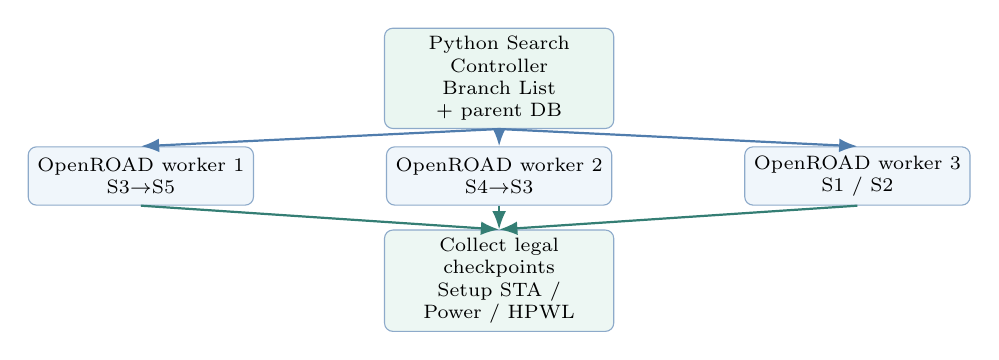
\begin{tikzpicture}[>=Latex,font=\scriptsize]
    \tikzset{b/.style={draw=AccentBlue!65,fill=SoftBlue!70,rounded corners=3pt,text width=2.70cm,minimum height=.67cm,align=center,inner sep=3pt},
              w/.style={b,text width=2.65cm,minimum height=.74cm}}
    \node[b,fill=SoftMint!85](controller) at (4.55,0) {Python Search Controller\\Branch List + parent DB};
    \node[w](w1) at (0,-1.24) {OpenROAD worker 1\\S3$\rightarrow$S5};
    \node[w](w2) at (4.55,-1.24) {OpenROAD worker 2\\S4$\rightarrow$S3};
    \node[w](w3) at (9.10,-1.24) {OpenROAD worker 3\\S1 / S2};
    \foreach \n in {w1,w2,w3}{\draw[->,AccentBlue,thick](controller.south)--(\n.north);}
    \node[b,fill=SoftMint!70](merge)at(4.55,-2.57){Collect legal checkpoints\\Setup STA / Power / HPWL};
    \foreach \n in {w1,w2,w3}{\draw[->,Accent,thick](\n.south)--(merge.north);}
  \end{tikzpicture}
  \end{center}
  \vspace{.20cm}
  \begin{columns}[T,onlytextwidth]
    \begin{column}{.48\textwidth}
      \smallpanel{panelblue}{Worker Responsibilities}{Apply ECO policy, legalize placement, update parasitics, collect full-design QoR, and save a restorable checkpoint.}
    \end{column}
    \begin{column}{.48\textwidth}
      \smallpanel{panelmint}{Controller Responsibilities}{Bound workers by available resources; update global best and Branch List using consistent QoR results.}
    \end{column}
  \end{columns}
\end{frame}


% DETAIL 10 / 10 | DC vs. ABC Synthesis Stages
\renewcommand{\slidenavigation}{\hyperlink{details-index}{\beamerbutton{Details index}}\hspace{.12cm}\hyperlink{summary-6}{\beamerreturnbutton{Summary 6}}}
\renewcommand{\slideposition}{Detail 10 / 10}
\begin{frame}[label=detail-dc-abc]{Design Compiler vs. ABC: Logic Synthesis Stages}
  \vspace{.02cm}\slidesubtitle{D10 / Logic Synthesis}\par\vspace{.08cm}
  \vspace{.18cm}
  \centering
  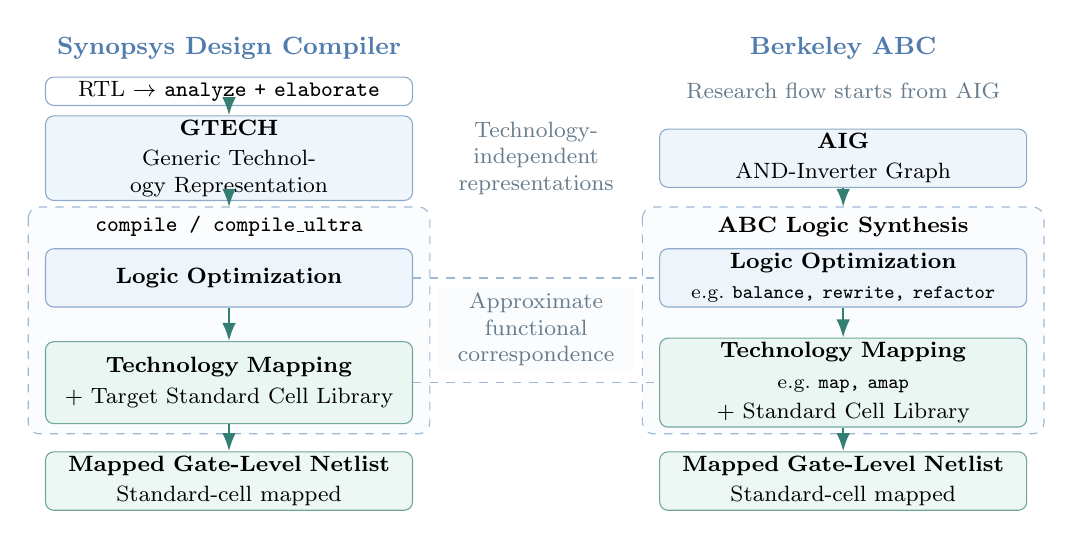
\begin{tikzpicture}[>=Latex,font=\footnotesize]
    \tikzset{
      stage/.style={draw=AccentBlue!65,fill=SoftBlue!72,rounded corners=3pt,
        text width=4.45cm,minimum height=.55cm,align=center,inner xsep=3pt,inner ysep=1.5pt},
      opt/.style={stage,fill=SoftBlue!80,minimum height=.74cm},
      mapping/.style={stage,draw=Accent!70,fill=SoftMint!85,minimum height=1.04cm},
      flow/.style={->,Accent,thick},
      cue/.style={dashed,AccentBlue!55,line width=.6pt}
    }
    \node[font=\small\bfseries,text=AccentBlue] at (0,0) {Synopsys Design Compiler};
    \node[font=\small\bfseries,text=AccentBlue] at (7.8,0) {Berkeley ABC};
    \node[stage,fill=white,minimum height=.32cm,font=\footnotesize] (front) at (0,-.55)
      {RTL $\rightarrow$ \texttt{analyze + elaborate}};
    \node[font=\footnotesize,text=Muted] at (7.8,-.55) {Research flow starts from AIG};
    \node[stage] (gtech) at (0,-1.40)
      {\textbf{GTECH}\\[1.5pt]{\footnotesize Generic Technology Representation}};
    \node[stage] (aig) at (7.8,-1.40)
      {\textbf{AIG}\\[1.5pt]{\footnotesize AND-Inverter Graph}};
    \draw[flow] (front.south)--(gtech.north);
    \node[font=\footnotesize,text=Muted,align=center,text width=2.6cm] at (3.9,-1.40)
      {Technology-independent\\representations};
    % Separate containers: these are independent tool flows, not a conversion.
    \foreach \x in {0,7.8}{
      \draw[draw=AccentBlue!55,dashed,rounded corners=4pt,fill=SoftBlue!25]
        (\x-2.55,-2.02) rectangle (\x+2.55,-4.90);
    }
    \node[font=\footnotesize\ttfamily\bfseries] at (0,-2.27) {compile / compile\_ultra};
    \node[font=\footnotesize\bfseries] at (7.8,-2.27) {ABC Logic Synthesis};
    \node[opt] (dcopt) at (0,-2.92) {\textbf{Logic Optimization}};
    \node[opt] (abcopt) at (7.8,-2.92)
      {\textbf{Logic Optimization}\\[1.5pt]{\scriptsize e.g.\ \texttt{balance, rewrite, refactor}}};
    \node[mapping] (dcmap) at (0,-4.25)
      {\textbf{Technology Mapping}\\[1.5pt]{\footnotesize + Target Standard Cell Library}};
    \node[mapping] (abcmap) at (7.8,-4.25)
      {\textbf{Technology Mapping}\\[1.5pt]{\scriptsize e.g.\ \texttt{map, amap}}\\[1.5pt]{\footnotesize + Standard Cell Library}};
    \draw[flow] (gtech.south)--(0,-2.02);
    \draw[flow] (aig.south)--(7.8,-2.02);
    \draw[flow] (dcopt.south)--(dcmap.north);
    \draw[flow] (abcopt.south)--(abcmap.north);
    % Dashed guides deliberately have no arrowheads: correspondence, not data flow.
    \draw[cue] (dcopt.east)--(abcopt.west);
    \draw[cue] (dcmap.east)--(abcmap.west);
    \node[fill=Paper,text=Muted,font=\footnotesize,align=center,text width=2.35cm,
      inner sep=2pt] at (3.9,-3.58) {Approximate functional\\correspondence};
    \node[stage,draw=Accent!70,fill=SoftMint!70] (dcout) at (0,-5.50)
      {\textbf{Mapped Gate-Level Netlist}\\[1.5pt]{\footnotesize Standard-cell mapped}};
    \node[stage,draw=Accent!70,fill=SoftMint!70] (abcout) at (7.8,-5.50)
      {\textbf{Mapped Gate-Level Netlist}\\[1.5pt]{\footnotesize Standard-cell mapped}};
    \draw[flow] (dcmap.south)--(dcout.north);
    \draw[flow] (abcmap.south)--(abcout.north);
  \end{tikzpicture}\par
\end{frame}

\end{document}
